% Propietario conservado: /Users/ruben/Documents/New project/output/EXTREMA_MEDIA_RAZON_RECIPROCIDAD_ES_EN_20260918/ARTICULO/ES/source/sections/excepcional.tex
\section{Prolongación excepcional: de la incidencia dodecafásica a Moonshine}
\label{x_reciprocidad:exc:seccion}

La expresión numérica no agota el estado que la ha generado. En la
construcción precedente, APP conserva las dos hojas y la división con
residuo y cociente; el TRIT determina el régimen local y su orientación;
el TPK compone selección, transporte, acarreo, memoria y retorno. La
lectura arquimediana contrae cilindros compatibles. La lectura que ahora
estudiamos conserva, en cambio, la incidencia de las posiciones y su
transporte entre marcos. Ambas parten del mismo estado aritmético con
memoria de trayectoria. No se
reconstruye una geometría excepcional a partir de los decimales finales
de $\pi$, $\varphi$, $e$ o $\alpha$.

Este punto permite precisar el sentido de la prolongación
$\alpha/K\longrightarrow\text{incidencia excepcional}$. La flecha no
afirma que un número real aislado determine un código, un retículo o un
grupo. Transporta el registro dodecafásico y los datos firmados que han
intervenido en la determinación de $\alpha$, junto con las palabras y los
marcos procedentes de APP--TRIT--TPK. En particular, el registro ordenado
$K$ puede recuperarse desde su constante racional $\kappa$ con las
convenciones de base, longitud y origen ya fijadas. La proyección a un
soporte conserva, en cambio, sólo las incidencias seleccionadas.
Por su parte, $K_{\rm ph}$
designa otra lectura, de memoria reducida, posterior a la holonomía
$\Gamma_9$.

La exposición separa tres operaciones matemáticas: construir los objetos
finitos y sus mapas; prolongarlos a un retículo y a un álgebra de operadores
de vértice; reconocer después los objetos obtenidos mediante los teoremas
clásicos pertinentes. Los nombres Paley, Witt, Mathieu, Golay, Leech y
Monstruo designan esos reconocimientos y las realizaciones explícitas
que los hacen verificables. No son selectores retrospectivos de las
semillas ni de los coeficientes de la generación.


% BEGIN OWNER /Users/ruben/Documents/New project/output/EXTREMA_MEDIA_RAZON_RECIPROCIDAD_ES_EN_20260918/ARTICULO/ES/source/sections/revision_incidencia_argumento.tex
El argumento comienza con la compatibilidad de prefijos y marcos,
construye el código ternario y determina la bandera mediante \(K\) y el
registro firmado de \(\alpha\). La incidencia marcada selecciona después
el origen reticular y el vecino de Leech. El último paso realiza el álgebra
de vértices y sus automorfismos. En cada etapa se precisará qué estructura
se conserva: combinaciones lineales, soportes, clases discriminantes, forma
bilineal o producto graduado. Las explicaciones de la función de \(K\),
de la normalización y del origen de norma \(54\) acompañan sus respectivas
construcciones en las secciones \ref{x_reciprocidad:exc:bandera} y \ref{x_reciprocidad:exc:leech}.

% END OWNER




\subsection{Compatibilidad de las realizaciones arquimediana e incidencial}
\label{x_reciprocidad:exc:doble-lectura}

Sea $X_n^{\rm cal}$ el espacio de prefijos admisibles de longitud $n$ del
estado aritmético con memoria de trayectoria, con truncaciones
$p_{n,m}:X_n^{\rm cal}\to X_m^{\rm cal}$ para $m\leq n$. El superíndice
recuerda que se conserva el marco inicial declarado y su transporte, no
que se ajuste un parámetro contra un valor experimental. Escribimos
$(w_j,f_j)$ para la palabra visible de seis trits y el marco en el paso
$j$. Los marcos satisfacen una ley causal
\[
 f_{j+1}=g_j(x)f_j,
\]
donde $g_j(x)$ depende del prefijo ya construido. En consecuencia, una
prolongación no altera los marcos anteriores.

La cadena
\[
 w_6\longrightarrow w_{12}\longrightarrow w_{18}
 \longrightarrow w_{24}\longrightarrow w_{30}
 \longrightarrow R_{36}\longrightarrow G_9
\]
se conserva en esta lectura. El retorno de la fase no reinicia ni el
marco ni la memoria del estado. Asimismo, se mantienen distintos el
censo de $468$ emisiones decimales, las $243$ palabras visibles de seis
trits y el ambiente $\mathbb F_3^6$, de $729$ palabras. El ambiente se
utilizará para construir un código lineal; no sustituye al dominio
admisible de emisiones.

La lectura arquimediana toma, para un bloque $b$ de seis trits, su
dirección entera $\nu(b)\in\{0,\ldots,728\}$. Un prefijo determina
\[
 q_n=m+\sum_{j=0}^{n-1}\frac{\nu(b_j)}{729^{j+1}},
 \qquad I_n=[q_n,q_n+729^{-n}].
\]
La compatibilidad de prefijos da cilindros encajados cuyo diámetro tiende
a cero. Su clase de Cauchy pertenece primero a la completación interna
$\mathbb R_{\rm HMT}$; su identificación posterior con la recta real
usual no interviene en la elección de los bloques.

Para la lectura incidencial introducimos, sobre el mismo prefijo, el
mapa de gráfico
\begin{equation}
 \gamma_A:\mathbb F_3^6\longrightarrow\mathbb F_3^{12},
 \qquad w\longmapsto(w,wA).
 \label{x_reciprocidad:exc:gamma}
\end{equation}
Las palabras se escriben como vectores fila. Si $A^f=fAf^{-1}$, el
cambio de marco satisface la identidad concreta
\begin{equation}
 \gamma_{A^f}(wf^{-1})
   =\gamma_A(w)(f^{-1}\oplus f^{-1}).
 \label{x_reciprocidad:exc:covariancia}
\end{equation}
El codominio calibrado conserva $f$ junto a la palabra codificada.
Definimos entonces
\begin{equation}
 Q_n(x)=\bigl((f_j,\gamma_{f_jA_Wf_j^{-1}}(w_j))\bigr)_{0\leq j<n}.
 \label{x_reciprocidad:exc:qn}
\end{equation}

\begin{proposition}[Compatibilidad y prolongación de la lectura incidencial]
\label{x_reciprocidad:exc:limite-inverso}
Si $r_{n,m}$ trunca las sucesiones codificadas, se cumple
\[
 r_{n,m}Q_n=Q_m p_{n,m}.
\]
Por tanto, los $Q_n$ determinan un único mapa $Q_\infty$ entre los
respectivos límites inversos. En cada marco, el mapa conserva exactamente
la palabra visible, pues $\operatorname{pr}_1\gamma_A=\operatorname{id}$.
\end{proposition}

\begin{proof}
Dos prefijos compatibles tienen las mismas palabras y los mismos
operadores de transporte hasta el índice $m-1$. Tienen, por inducción,
los mismos marcos en esos índices. Las primeras $m$ componentes de
\eqref{x_reciprocidad:exc:qn} coinciden, lo que prueba el cuadrado. La propiedad
universal del límite inverso da $Q_\infty$. La afirmación de recuperación
es la proyección sobre las seis primeras coordenadas de cada gráfico.
\end{proof}

Esta inyectividad local tiene un dominio preciso. No demuestra que
$Q_\infty$ recupere toda la memoria profunda del estado TPK si sólo se
ha retenido la sucesión de palabras visibles y marcos. Mucho menos
demuestra inyectividad después de pasar de palabras a soportes.
Además, un cambio general de base en $\operatorname{GL}_6(\mathbb F_3)$
no conserva por sí mismo el peso de Hamming ordinario. En una carta
general se transportan también la incidencia y la métrica de la carta
inicial. Los cálculos de soportes que siguen se realizan en la carta
Paley declarada; los relabelados monomiales conservan directamente su
interpretación coordenada.

\subsection{La realización finita y el código ternario}
\label{x_reciprocidad:exc:paley-codigo}

El operador elíptico del TRIT admite la siguiente realización finita en
la carta de seis posiciones. Éstas coordinatizan las seis unidades
$\{1,2,4,5,7,8\}$ módulo nueve, conservadas por el transporte modular.
Sobre $\mathbb P^1(\mathbb F_5)$, una vez
declarado el orden $\infty,0,1,2,3,4$, sea $C$ la matriz con diagonal
nula, $C_{\infty,a}=C_{a,\infty}=1$ y
$C_{a,b}=\chi(b-a)$ en las cinco posiciones finitas. Aquí
$\chi(1)=\chi(4)=1$, $\chi(2)=\chi(3)=-1$ y $\chi(0)=0$.
Es una realización en coordenadas de la estructura cuadrática ya
transportada; la identificación de las seis posiciones con la recta
proyectiva es un dato de carta, no una nueva entrada numérica en el
generador.

Las identidades de la suma cuadrática dan $C^2=5I_6$. Al reducir módulo
tres obtenemos
\begin{equation}
 A_W=
 \begin{pmatrix}
 0&1&1&1&1&1\\
 1&0&1&2&2&1\\
 1&1&0&1&2&2\\
 1&2&1&0&1&2\\
 1&2&2&1&0&1\\
 1&1&2&2&1&0
 \end{pmatrix},
 \qquad A_W^2=2I_6=-I_6.
 \label{x_reciprocidad:exc:aw}
\end{equation}
La igualdad cuadrática realiza el régimen elíptico; no identifica el
cuerpo $\mathbb F_3$ con una realización arquimediana de la unidad
imaginaria. Son realizaciones distintas de una relación operatoria
común, con sus correspondientes dominios.

\Needspace{8\baselineskip}
\begin{definition}[Código de la carta dodecafásica]
\label{x_reciprocidad:exc:codigo}
El código ternario asociado a \eqref{x_reciprocidad:exc:aw} es
\[
 C_W=\{(w,wA_W):w\in\mathbb F_3^6\}
       \subset\mathbb F_3^{12}.
\]
Su conjunto de hexadas es
\[
 \mathcal H=
 \{\operatorname{supp}(c):c\in C_W,
                           \operatorname{wt}(c)=6\}.
\]
\end{definition}

\begin{proposition}[Autodualidad, distancia y diseño de Witt]
\label{x_reciprocidad:exc:codigo-witt}
El código $C_W$ es autodual de parámetros $[12,6,6]_3$. Su enumerador
de pesos es
\begin{equation}
 \sum_{c\in C_W}z^{\operatorname{wt}(c)}
   =1+264z^6+440z^9+24z^{12}.
 \label{x_reciprocidad:exc:enumerador}
\end{equation}
El conjunto $\mathcal H$ tiene $132$ elementos y constituye un sistema
$S(5,6,12)$: cada conjunto de cinco posiciones está contenido en una
única hexada.
\end{proposition}

\begin{proof}
La matriz generadora $[I_6\mid A_W]$ tiene rango seis y, por simetría
de $A_W$, satisface
\[
 [I_6\mid A_W][I_6\mid A_W]^{\mathsf T}
   =I_6+A_W^2=0.
\]
El código es autoortogonal de dimensión mitad de la longitud y, por
tanto, autodual. La evaluación finita de las $3^6$ palabras da
\eqref{x_reciprocidad:exc:enumerador}; es una enumeración sobre la matriz explícita,
sin valores reales ni objetivos externos. En particular, la distancia
mínima es seis.

Si dos palabras de peso seis tienen el mismo soporte, entre sus seis
cocientes de coordenadas no nulas uno de los signos $1,-1$ aparece al
menos tres veces. Restando el múltiplo correspondiente se obtendría
una palabra no nula de peso a lo sumo tres, imposible. Luego un soporte
corresponde exactamente a la pareja $\{c,-c\}$ y hay $264/2=132$
soportes. Si dos soportes distintos compartieran cinco posiciones,
el mismo argumento cancelaría al menos tres coordenadas de una unión
de tamaño siete, produciendo peso a lo sumo cuatro. Por ello una
quintupla pertenece a lo sumo a una hexada. Finalmente,
\[
 132\binom65=792=\binom{12}5,
\]
de modo que pertenece a una y sólo una.
\end{proof}

El reconocimiento posterior es el código de Golay ternario extendido y
el pequeño diseño de Witt \cite{x_reciprocidad:conwaysloane}. La prueba anterior explica qué objeto se
reconoce. No reemplaza la genealogía APP--TRIT--TPK por una búsqueda
entre códigos conocidos.

\subsection{Bandera dodecafásica asociada a \texorpdfstring{$K$ y $\alpha$}{K y alfa}}
\label{x_reciprocidad:exc:bandera}


% BEGIN OWNER /Users/ruben/Documents/New project/output/EXTREMA_MEDIA_RAZON_RECIPROCIDAD_ES_EN_20260918/ARTICULO/ES/source/sections/incidencia_registro.tex
\paragraph{Articulación de las coordenadas regionales y la incidencia de clausura.}
\label{x_reciprocidad:inc-ampl-articulacion}
La función de esta prolongación se comprende a partir de una distinción
entre tres operaciones: conservar un registro, evaluar una coordenada y
extraer una relación de incidencia. Las tres actúan sobre información
producida por APP--TRIT--TPK. Su articulación hace explícita la tesis
estructural del artículo: una realización numérica posee una procedencia
operatoria, y determinados datos de esa procedencia admiten, además, una
realización combinatoria y reticular. Las ecuaciones permiten seguir ambos
recorridos con sus dominios y con la información que permanece en cada uno.

El punto de partida es el estado terminal con sus prolongaciones
compatibles. En él se conservan los residuos y cocientes de las dos hojas
APP, el régimen y la orientación TRIT, y el transporte TPK con su memoria.
Las regiones de clausura, propagación y autoescala se determinan en ese
dominio antes de que sus lectores establezcan las coordenadas
$\pi,e,\varphi$. Al mismo tiempo, el registro orientado de las doce
ventanas determina el vector firmado $U$. La aparición posterior de $K$
procede de la transformación integral demostrada en
\S\ref{x_reciprocidad:subsec:k-hadamard}:
\begin{equation}
 U=\mathcal H_{12}K,\qquad
 K=\frac14\mathcal H_{12}U,\qquad
 \mathcal H_{12}^{2}=4I_{12}.
 \label{x_reciprocidad:inc-ampl-registro}
\end{equation}
La congruencia que define $\mathcal L_H$ garantiza la integralidad de
la inversa. De este modo, $K$ constituye una coordenatización reversible
del registro firmado en la subred pertinente. Sus posiciones conservan el
orden de fase; sus diferencias $D_3K,D_4K$ conservan las relaciones
transversales; la suma $Q(K)$ determina la componente uniforme. Esa
estructura explica por qué el registro interviene tanto en la composición
numérica como en la selección de una configuración de frontera.

La evaluación periódica
\[
 K\longmapsto\kappa_{\mathrm{per}}
 =\frac{\sum_{m=1}^{12}K_m1000^{12-m}}{1000^{12}-1}
\]
mantiene recuperables los doce bloques cuando se fijan base, longitud y
origen de fase. La extracción de un soporte realiza una operación
diferente: conserva la pertenencia de cada posición a una clase definida
por un umbral y agrupa los registros que tienen el mismo soporte. La
distinción entre estas dos aplicaciones resulta decisiva. La precisión
escalar de $\kappa_{\mathrm{per}}$ y la incidencia de $B_K$ son dos
contenidos matemáticos específicos, relacionados mediante el registro
completo del que proceden.


% END OWNER


En el marco heredado del registro dodecafásico, los datos son
\begin{align}
 K={}&(234,543,140,729,659,824,621,\mathtt{058},914,794,146,601),
 \label{x_reciprocidad:exc:k}\\
 w_\pi={}&010211, &w_e={}&201101,\nonumber\\
 w_\varphi={}&121200, &w_{\rm APP}={}&022020.\nonumber
\end{align}
Al aplicar $\gamma_{A_W}$ se obtienen las siguientes incidencias:
\begin{align*}
 P_\pi&=\{2,4,5,6,7,8,9,10,11\},\\
 H_e&=\{1,3,4,6,9,10\},\\
 H_\varphi&=\{1,2,3,4,7,9\},\\
 H_{\rm APP}&=\{2,3,5,10,11,12\}.
\end{align*}
La primera es el soporte de una palabra de peso nueve; las otras tres
son hexadas. El registro aporta, por su lectura de bloque alto,
\begin{equation}
 B_K=\{i:K_i\geq729\}=\{4,6,9,10\}=H_e\cap P_\pi.
 \label{x_reciprocidad:exc:bk}
\end{equation}
El entero $729$ señala aquí una frontera del formato de bloques
declarado. No se identifica por el mero cardinal con el ambiente
ternario usado en \eqref{x_reciprocidad:exc:codigo}. En este registro concreto, todos
los umbrales enteros entre $660$ y $729$ producen el mismo soporte:
el soporte no recupera el umbral ni los doce bloques.

La vía aritmética de $\alpha$ conserva, antes del acarreo, el vector
firmado
\begin{equation}
 Z_0=(7,297,353,-430,-715,-1199,-3,286,-894,-528,380,663).
 \label{x_reciprocidad:exc:precarry}
\end{equation}
Su soporte negativo es
\begin{equation}
 H^-_\alpha=\{4,5,6,7,9,10\}.
 \label{x_reciprocidad:exc:halpha}
\end{equation}
No se extraen estos signos de la expansión decimal del escalar
$\alpha$; se conservan en el estado que precede a su expresión numérica.


% BEGIN OWNER /Users/ruben/Documents/New project/output/EXTREMA_MEDIA_RAZON_RECIPROCIDAD_ES_EN_20260918/ARTICULO/ES/source/sections/incidencia_normalizacion.tex
\paragraph{La normalización de alfa y su configuración firmada.}
\label{x_reciprocidad:inc-ampl-clausura}
La coordenada de $\alpha$ se determina en la vía posicional mediante la
composición de los bloques regionales y del registro dodecafásico. Antes
de la división posicional, la combinación orientada tiene componentes
$Z_j=P_j+E_j-\Phi_j-K_j^{\mathrm{per}}$ y el balance con cociente entrante
es $s_j=Z_j+c_{j+1}$. La normalización satisface
\begin{equation}
 A_j=s_j-1000c_j=Z_j+c_{j+1}-1000c_j,\qquad 0\leq A_j<1000.
 \label{x_reciprocidad:inc-ampl-normalizacion}
\end{equation}
Esta identidad conserva simultáneamente el bloque normalizado y la
contribución del cociente transportado. El límite de los prefijos
compatibles determina la coordenada escalar de la clausura. La
configuración firmada conserva, por su parte, qué posiciones de la
combinación anterior a la normalización presentan defecto negativo.
En la ventana inicial, esa configuración es el vector $Z_0$ de
\eqref{x_reciprocidad:exc:precarry}, y su soporte negativo es $H^-_\alpha$.

Así quedan definidos dos contenidos de una misma operación. La
normalización posicional determina una coordenada real mediante sus
restos y cocientes compatibles; el soporte negativo determina una
configuración de posiciones en el ciclo de doce componentes. El signo se
refiere al balance de registros anterior a la normalización. Su lectura
incidencial permanece disponible porque el estado conserva ese balance
junto con el resultado normalizado. Esta articulación corresponde a la
vía posicional demostrada; la comparación con los operadores analíticos
de vacancias conserva el alcance preciso establecido en el capítulo de
$\alpha$.

% END OWNER


\begin{proposition}[Coincidencia de los dos selectores de la bandera]
\label{x_reciprocidad:exc:selector-bandera}
Dentro de $\mathcal H$, el soporte \eqref{x_reciprocidad:exc:halpha} es la única hexada
$H$ que satisface
\[
 B_K\subset H\subset P_\pi,
 \qquad
 (|H\cap H_e|,|H\cap H_\varphi|,|H\cap H_{\rm APP}|)=(4,3,2).
\]
Así, la lectura firmada y la lectura incidencial seleccionan la misma
bandera $B_K\subset H^-_\alpha$.
\end{proposition}

\begin{proof}
Las cuatro hexadas que contienen $B_K$ se obtienen añadiendo,
respectivamente, los pares
\[
 \{1,3\},\qquad\{2,11\},\qquad\{5,7\},\qquad\{8,12\}.
\]
Sólo los pares segundo y tercero están contenidos en $P_\pi$. Para el
segundo, la intersección con $H_\varphi$ tiene tamaño tres y con
$H_{\rm APP}$ tamaño tres; no cumple la última condición. Para el
tercero, las tres intersecciones tienen tamaños $4,3,2$. Este último
produce precisamente el soporte negativo de \eqref{x_reciprocidad:exc:precarry}.
\end{proof}

Conviene conservar tanto la bandera como su marco marcado:
\[
 \mathcal I_*=(B_K\subset H^-_\alpha),\qquad
 \widetilde{\mathcal I}_*
   =(\mathcal I_*;P_\pi,H_e,H_\varphi,H_{\rm APP}).
\]
Las operaciones de unión, intersección y diferencia son equivariantes
bajo un relabelado simultáneo del diseño. La clase marcada, y no los
números de las posiciones tomados aisladamente, es el objeto transportado.

\begin{lemma}[Origen seleccionado por la incidencia marcada]
\label{x_reciprocidad:exc:origen}
Para el marco anterior,
\[
 o_*=(H_e\cap H_\varphi)
           \setminus(H^-_\alpha\cup H_{\rm APP})=\{1\}.
\]
La regla es equivariante bajo todo automorfismo aplicado simultáneamente
a los datos de $\widetilde{\mathcal I}_*$.
\end{lemma}

\begin{proof}
La primera intersección es $\{1,3,4,9\}$. La unión que se sustrae
contiene $3,4,9$ y no contiene $1$. La equivariancia se sigue de que una
biyección conmuta con las operaciones de conjuntos.
\end{proof}

Este origen seleccionará una dirección del vecino reticular cuando se
declaren la métrica $A_2$ y la cámara positiva. La incidencia por sí sola
no contiene esa métrica. El paso reticular conservará explícitamente
ambos datos.


% BEGIN OWNER /Users/ruben/Documents/New project/output/EXTREMA_MEDIA_RAZON_RECIPROCIDAD_ES_EN_20260918/ARTICULO/ES/source/sections/incidencia_bandera.tex
\paragraph{De la codificación ternaria a la bandera marcada.}
\label{x_reciprocidad:inc-ampl-bandera}
Las regiones aportan también los códigos $w_\pi,w_e,w_\varphi$ y
$w_{\rm APP}$ en el marco heredado. La aplicación
\[
 \gamma_{A_W}:w\longmapsto(w,wA_W)
\]
conserva la palabra de seis componentes como primera coordenada y añade
su transformación por $A_W$. La relación $A_W^2=-I_6$ fija la
compatibilidad cuadrática de esta realización. El paso siguiente,
$c\mapsto\operatorname{supp}(c)$, conserva las posiciones no nulas.
En las palabras de peso seis, el soporte identifica exactamente la pareja
$\{c,-c\}$, como prueba la distancia mínima del código. De esta forma,
el cociente por signo produce las hexadas, mientras el código completo
sigue disponible para las operaciones que requieren sus símbolos.

En esta carta, las dos construcciones de la cuaterna coinciden:
\begin{equation}
 \{i:K_i\geq729\}
 =H_e\cap P_\pi=B_K=\{4,6,9,10\}.
 \label{x_reciprocidad:inc-ampl-cuaterna}
\end{equation}
El lado izquierdo procede de una comparación entera de los componentes
de $K$; el derecho, de la intersección de los soportes codificados de
propagación y clausura. El umbral pertenece a la carta de bloques
declarada y permanece explicitado en la definición del lector. El
registro íntegro conserva los valores sobre los que actúa, incluso cuando
distintos umbrales producen el mismo subconjunto. La igualdad expresa,
por tanto, una compatibilidad entre aplicaciones especificadas.

El soporte $H^-_\alpha$ completa esa cuaterna hasta una hexada. La
condición de pertenencia al soporte $P_\pi$, junto con los tamaños de
intersección $(4,3,2)$ respecto de $H_e,H_\varphi,H_{\rm APP}$,
selecciona una única hexada. Las pruebas siguientes reúnen las dos
determinaciones: la obtenida mediante el signo de $Z_0$ y la obtenida
mediante incidencia. El resultado se organiza como
\begin{equation}
 \widetilde{\mathcal I}_*
 =\bigl(B_K\subset H^-_\alpha;
         P_\pi,H_e,H_\varphi,H_{\rm APP}\bigr).
 \label{x_reciprocidad:inc-ampl-marco}
\end{equation}
La inclusión es la bandera; los cuatro soportes adicionales constituyen
su marco marcado. Las permutaciones simultáneas transportan el marco y
conservan sus inclusiones e intersecciones. La información relevante reside
en esta configuración transportada y en su clase de isomorfía.

Las cinco regiones de $\pi$ recuperan aquí su diferenciación interna.
Comparten $w_\pi$ como código ternario visible, pero conservan emisiones,
firmas y multiplicidades distintas. En la realización binaria sobre una
dodecada marcada, la región transversal corresponde a la octada cuya
intersección con la dodecada es la cuaterna; las otras cuatro regiones
corresponden a las elevaciones de las cuatro hexadas de su estrella. La
región negativa queda distinguida por $H^-_\alpha$ y el orden de carta
individualiza las tres regiones positivas. Esta correspondencia conserva
los papeles regionales y la distribución $432+4\cdot144=1008$, además
de realizar la partición incidencial $1+4$.

% END OWNER


\subsection{Entrelazamiento isométrico de las representaciones de incidencia}
\label{x_reciprocidad:exc:entrelazador}

La incidencia define un mapa lineal cuya acción puede comprobarse
posición por posición:
\begin{equation}
 I:\mathbb R^{12}\longrightarrow\mathbb R^{\mathcal H},
 \qquad (Iv)(H)=\sum_{p\in H}v_p.
 \label{x_reciprocidad:exc:incidencia}
\end{equation}
Sea $V_{11}=\mathbf1^\perp\subset\mathbb R^{12}$. Las dos realizaciones
euclídeas son aquí lenguajes posteriores para el mismo diseño finito.

\begin{proposition}[Isometría de la pantalla dodecafásica]
\label{x_reciprocidad:exc:isometria}
Se cumple
\[
 I^{\mathsf T}I=36I_{12}+30J_{12},
\]
donde $J_{12}$ es la matriz cuyas entradas son uno. En consecuencia,
\[
 U_W=\frac16 I\big|_{V_{11}}:
 V_{11}\xrightarrow{\ \sim\ }E_{\rm inc}:=I(V_{11})
\]
es una isometría equivariante para las acciones por permutación de los
automorfismos del diseño.
\end{proposition}

\begin{proof}
Cada punto pertenece a
$r=\binom{11}{4}/\binom54=66$ hexadas, y cada pareja a
$\lambda_2=\binom{10}{3}/\binom43=30$. Son, respectivamente, las
entradas diagonales y no diagonales de $I^{\mathsf T}I$. Sobre
$\mathbf1^\perp$, el término $J_{12}$ se anula y queda $36I$.
Por último, si $g$ es un automorfismo, $p\in H$ equivale a
$g(p)\in g(H)$; por ello $I\rho_{12}(g)=\rho_{\mathcal H}(g)I$.
\end{proof}

La información de incidencia también tiene una lectura espectral
concreta. Definamos
\[
 G_{H,H'}=\binom{|H\cap H'|}{4}.
\]

\Needspace{8\baselineskip}
\begin{lemma}[Acción del núcleo de intersección]
\label{x_reciprocidad:exc:espectro}
Si $J_{132,12}$ es la matriz rectangular de unos,
\[
 GI=30I+15J_{132,12}.
\]
Por tanto, $G$ actúa por el escalar $30$ en $E_{\rm inc}$.
\end{lemma}

\begin{proof}
La entrada $(H,p)$ de $GI$ cuenta parejas $(T,H')$ con
$T\subset H\cap H'$, $|T|=4$ y $p\in H'$. Si $p\in H$, hay diez
cuaternas $T$ que contienen $p$, cada una contenida en cuatro hexadas,
y cinco que no lo contienen, cada una con una única extensión de la
quintupla $T\cup\{p\}$. El total es $10\cdot4+5=45$.
Si $p\notin H$, las quince cuaternas de $H$ dan una extensión cada
una: el total es $15$. De ahí la identidad. El término rectangular
se anula en $V_{11}$.
\end{proof}

Aquí sí existe un entrelazador material: tiene dominio, codominio,
entradas y normalización determinados. Por ejemplo, cualquier
proyector ortogonal $P$ ya construido sobre $V_{11}$ se transporta a
$Q=U_WPU_W^*$ sobre $E_{\rm inc}$, con
$U_WP=QU_W$. Esta afirmación no identifica por su sola traza a todos
los operadores que actúan en esos espacios.


% BEGIN OWNER /Users/ruben/Documents/New project/output/EXTREMA_MEDIA_RAZON_RECIPROCIDAD_ES_EN_20260918/ARTICULO/ES/source/sections/k_direccion_dimensional.tex
\subsection{La dirección seleccionada por el registro dodecafásico}
\label{x_reciprocidad:exc:k-direccion}

El registro \(K\) tiene una función geométrica que complementa su
evaluación racional y su lectura de soportes. Una vez construida la
representación de las doce posiciones, sus componentes determinan una
dirección en el espacio de variaciones de media nula. La reducción
\(12\to11\) elimina el modo uniforme; la reducción siguiente
\(11\to10\) elimina la dirección que selecciona el propio registro.
Las dos operaciones tienen, por tanto, antecedentes diferentes.

Para declarar completamente la carta utilizada, consideremos el grupo
\(A_5\) de permutaciones pares de cinco objetos y el subgrupo
\(C_5=\langle(1\,2\,3\,4\,5)\rangle\). Las doce clases izquierdas
\(r_pC_5\) se ordenan mediante estos representantes, escritos como
listas de imágenes:
\[
\begin{array}{c|c@{\qquad}c|c}
p&r_p&p&r_p\\ \hline
1&(4,3,5,2,1)&7&(5,4,3,2,1)\\
2&(4,2,1,3,5)&8&(1,3,4,2,5)\\
3&(1,2,4,5,3)&9&(4,2,3,5,1)\\
4&(2,5,3,4,1)&10&(3,2,5,4,1)\\
5&(4,3,1,5,2)&11&(4,5,2,3,1)\\
6&(5,1,2,3,4)&12&(5,3,2,4,1).
\end{array}
\]
La acción por multiplicación izquierda define una representación
ortogonal \(\rho:A_5\to O(\RR^{12})\):
\(\rho(a)e_p=e_q\) cuando \(ar_pC_5=r_qC_5\).
Esta carta de representación actúa sobre el registro ya obtenido;
los caracteres del grupo no se utilizan para elegir sus doce valores.

Sean \(\chi_3\) los valores del carácter tridimensional
\[
\begin{array}{c|ccccc}
\text{clase}&1&2^2&3&5_a&5_b\\ \hline
\chi_3&3&-1&0&(1+\sqrt5)/2&(1-\sqrt5)/2.
\end{array}
\]
La clase \(5_a\) contiene el generador de \(C_5\) mostrado y
\(5_b\) contiene su cuadrado. Esta convención distingue los dos
sectores tridimensionales conjugados de la representación. Definimos
\begin{equation}
 P_3=\frac3{60}\sum_{a\in A_5}\chi_3(a^{-1})\rho(a),
 \qquad P_{11}=I_{12}-\frac1{12}J_{12}.
 \label{x_reciprocidad:eq:k-proyectores-incidencia}
\end{equation}
Ambas matrices quedan determinadas por sumas finitas en
\(\QQ(\sqrt5)\). La aparición de este cuerpo cuadrático pertenece
a la realización de la representación, posterior a la generación
regional de \(\varphi\).

\begin{lemma}[Proyección del registro sobre el sector tridimensional]
\label{x_reciprocidad:lem:k-sector-no-nulo}
Se tienen
\[
 P_3=P_3^{\mathsf T}=P_3^2,\quad
 P_3\mathbf1=0,\quad \operatorname{tr}P_3=3,
 \qquad P_3P_{11}=P_{11}P_3=P_3.
\]
Para el registro \eqref{x_reciprocidad:exc:k}, el vector
\begin{equation}
 u_K=P_3P_{11}K
 \label{x_reciprocidad:eq:k-vector-direccional}
\end{equation}
es no nulo. Su norma exacta es
\begin{equation}
 \lVert u_K\rVert^2
 =\frac{6638585+2275584\sqrt5}{20}>0.
 \label{x_reciprocidad:eq:k-norma-direccion}
\end{equation}
\end{lemma}
\begin{proof}
La suma de carácter en \eqref{x_reciprocidad:eq:k-proyectores-incidencia} es el
proyector isótipo. El carácter real y la sustitución \(a\mapsto a^{-1}\)
dan la simetría. La multiplicidad del sector en la acción sobre
\(A_5/C_5\) es la dimensión de sus vectores fijos por \(C_5\),
\[
 \frac15\left(3+2\frac{1+\sqrt5}{2}
                 +2\frac{1-\sqrt5}{2}\right)=1.
\]
Por ello el rango es tres. Su ortogonalidad al carácter trivial
da \(P_3\mathbf1=0\) y las dos composiciones con \(P_{11}\).
También pueden verificarse estas identidades multiplicando las
matrices de la suma finita.

Finalmente, \(\sum K_p=6263\) y la sustitución de las doce
componentes en esa misma suma da
\[
 \lVert u_K\rVert^2=K^{\mathsf T}P_3K
 =\frac1{20}\sum_{a\in A_5}
                \chi_3(a^{-1})K^{\mathsf T}\rho(a)K
 =\frac{6638585+2275584\sqrt5}{20}.
\]
Esta es una evaluación exacta de sesenta términos especificados,
reproducida por el certificado adjunto con aritmética racional
cuadrática. Los dos coeficientes positivos prueban la no nulidad.
\end{proof}

\begin{definition}[Dirección dodecafásica y complemento transversal]
La dirección seleccionada por \(K\) en la carta declarada es
\(\ell_K=\RR u_K\). Su complemento transversal dentro de
\(V_{11}=\mathbf1^\perp\) es
\[
 V_{10}(K)=V_{11}\cap u_K^\perp.
\]
\end{definition}

\begin{proposition}[Reducción ortogonal determinada por \(K\)]
\label{x_reciprocidad:prop:k-reduccion-diez}
El operador
\begin{equation}
 P_{10}(K)=P_{11}
       -\frac{u_Ku_K^{\mathsf T}}{\lVert u_K\rVert^2}
 \label{x_reciprocidad:eq:k-proyector-diez}
\end{equation}
es el proyector ortogonal de rango diez sobre \(V_{10}(K)\). Se cumple
\[
 V_{11}=\ell_K\mathbin{\oplus^{\perp}}V_{10}(K),
 \qquad P_{10}P_{11}=P_{10},\quad P_{10}u_K=0.
\]
\end{proposition}
\begin{proof}
Sea \(E_K=u_Ku_K^{\mathsf T}/\lVert u_K\rVert^2\). La
no nulidad demostrada garantiza que está definido. Es simétrico,
\(E_K^2=E_K\), tiene rango uno y, como \(u_K\in V_{11}\),
\(P_{11}E_K=E_KP_{11}=E_K\). De aquí
\[
 (P_{11}-E_K)^2=P_{11}-2E_K+E_K=P_{11}-E_K.
\]
Su imagen es \(V_{11}\cap u_K^\perp\) y su traza es
\(11-1=10\). La descomposición y las identidades restantes se
obtienen por proyección sobre los dos sumandos ortogonales.
\end{proof}

Este resultado precisa una función de \(K\) que su denominación como
registro no agotaba: además de representar reversiblemente datos
orientados y de seleccionar la tétrada \(B_K\), determina una
polarización lineal. La dirección depende del registro completo a
través de \(P_3K\), no únicamente de los cuatro puntos de su soporte.
Se ha mantenido así el orden registro, representación, dirección y
reducción dimensional (proposición~\ref{x_reciprocidad:prop:k-reduccion-diez}).

La transformación tiene una ley de covariancia precisa. Si se cambia
simultáneamente la carta por una matriz ortogonal de permutación \(S\),
\(K'=SK\) y \(P'_3=SP_3S^{-1}\), entonces
\[
 u_{K'}'=Su_K,\qquad P'_{10}(K')=SP_{10}(K)S^{-1}.
\]
Por otra parte, sustituir \(u_K\) por \(a u_K\), con \(a\ne0\),
no cambia \(E_K\). La dirección retiene una polarización y no
permite recuperar por sí sola ni la amplitud de \(u_K\) ni el
registro íntegro. La reversibilidad de \(\kappa\leftrightarrow K\)
permanece en su dominio propio.

La realización geométrica aquí establecida es una reducción de espacios
con producto interno. Su empleo posterior como dirección compacta
requiere transportar esta recta a la realización física correspondiente.
El apartado \ref{x_reciprocidad:exc:pantallas-dualidad} expone el mapa algebraico
que mantiene coordinadas esta reducción y la pantalla reticular.

% END OWNER


\subsection{La estrella de Witt y la generación de \texorpdfstring{$M_{12}$}{M12}}
\label{x_reciprocidad:exc:estrella}

\begin{definition}[Estrella sobre una cuaterna]
\label{x_reciprocidad:exc:def-estrella}
Para $B\in\binom{[12]}4$, la estrella de Witt es la familia de las
cuatro hexadas que contienen $B$. Sus pétalos son los pares $H\setminus B$.
La permutación $\sigma_B$ fija $B$ e intercambia los dos puntos de cada
pétalo.
\end{definition}

La existencia de cuatro hexadas se deduce de
\[
 \lambda_4=\frac{\binom81}{\binom21}=4.
\]
Dos pétalos no pueden compartir un punto, pues entonces dos hexadas
contendrían la misma quintupla. Son, por tanto, cuatro pares disjuntos
que particionan $[12]\setminus B$. Esta descripción no es una estrella
de cinco puntas ni una metáfora geométrica: es una incidencia
cuatro-a-uno del diseño.

\begin{figure}[htbp]
\centering
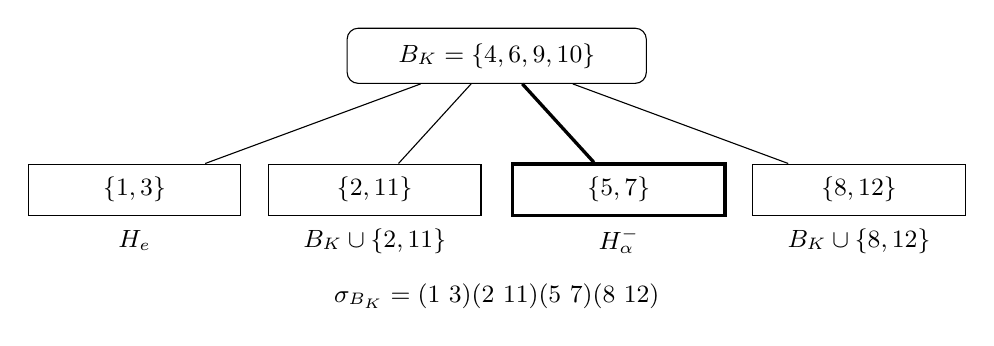
\begin{tikzpicture}[x=1cm,y=1cm, every node/.style={font=\small}]
 \node[draw,rounded corners,minimum width=3.8cm,minimum height=.7cm]
  (b) at (0,0) {$B_K=\{4,6,9,10\}$};
 \node[draw,minimum width=2.7cm,minimum height=.65cm]
  (p1) at (-4.6,-1.7) {$\{1,3\}$};
 \node[draw,minimum width=2.7cm,minimum height=.65cm]
  (p2) at (-1.55,-1.7) {$\{2,11\}$};
 \node[draw,very thick,minimum width=2.7cm,minimum height=.65cm]
  (p3) at (1.55,-1.7) {$\{5,7\}$};
 \node[draw,minimum width=2.7cm,minimum height=.65cm]
  (p4) at (4.6,-1.7) {$\{8,12\}$};
 \draw (b) -- (p1); \draw (b) -- (p2);
 \draw[very thick] (b) -- (p3); \draw (b) -- (p4);
 \node at (-4.6,-2.35) {$H_e$};
 \node at (-1.55,-2.35) {$B_K\cup\{2,11\}$};
 \node at (1.55,-2.35) {$H^-_\alpha$};
 \node at (4.6,-2.35) {$B_K\cup\{8,12\}$};
 \node at (0,-3.05)
  {$\sigma_{B_K}=(1\ 3)(2\ 11)(5\ 7)(8\ 12)$};
\end{tikzpicture}
\caption{La estrella concreta de la bandera dodecafásica. Cada línea
indica la unión de la cuaterna central con el par de su extremo; la
línea gruesa señala la hexada seleccionada también por los signos
anteriores al acarreo de $\alpha$. Los cuatro pares agotan las ocho
posiciones exteriores.}
\label{x_reciprocidad:exc:fig-estrella}
\end{figure}

\begin{proposition}[La familia de estrellas]
\label{x_reciprocidad:exc:m12}
Las $\binom{12}4=495$ permutaciones $\sigma_B$ preservan $\mathcal H$.
El grupo que generan tiene orden $95040$ y es el grupo de Mathieu
$M_{12}$ en su acción sobre el pequeño diseño de Witt.
\end{proposition}

\begin{proof}
La afirmación de preservación es una comprobación finita sobre las
$132$ hexadas de \eqref{x_reciprocidad:exc:codigo}: para cada cuaterna se construyen
los cuatro pétalos y se verifica
$\{\sigma_B(H):H\in\mathcal H\}=\mathcal H$.
La clausura por composición de estas permutaciones produce $95040$
elementos. En la enumeración lexicográfica basta añadir sucesivamente
seis estrellas no contenidas aún en el grupo; los órdenes intermedios
son $2,6,18,360,7920,95040$, y las $495$ estrellas pertenecen al grupo
final. El procedimiento, las seis permutaciones escritas mediante sus
listas de imágenes y la recurrencia de clausura se desarrollan en
\ref{iv:iv:apendice-estrellas}. Finalmente se aplica el reconocimiento
del grupo de automorfismos de $S(5,6,12)$ como $M_{12}$, cuyo orden es
$12\cdot11\cdot10\cdot9\cdot8=95040$.
\end{proof}

Una estrella individual genera un grupo cíclico de orden dos. No
genera por sí sola $M_{12}$, y menos aún el Monstruo. Tampoco la
existencia de $495$ generadores de un grupo de permutaciones prueba que
cada uno sea el transporte de un lazo específico del TPK. Esa afirmación
requiere el mapa de lazos correspondiente; el resultado aquí establecido
es la acción incidencial finita.

\begin{remark}[La igualdad de trazas no identifica operadores]
Sobre $V_{11}$, una estrella tiene espectro $+1$ con multiplicidad siete
y $-1$ con multiplicidad cuatro. Su traza normalizada es $3/11$.
Un proyector de rango tres en el mismo espacio tiene también traza
normalizada $3/11$, pero espectro $1^3,0^8$. No son conjugados: sus
polinomios mínimos y sus espectros son diferentes. El entrelazador
\eqref{x_reciprocidad:exc:incidencia} transporta operadores definidos; no convierte
esta coincidencia escalar en una equivalencia de operadores.
\end{remark}

\subsection{El residuo binario y las cinco regiones de \texorpdfstring{$\pi$}{pi}}
\label{x_reciprocidad:exc:cinco-regiones}

El siguiente reconocimiento utiliza el código de Golay binario
extendido $G_{24}$, de parámetros $[24,12,8]_2$. Sus pesos son
$0,8,12,16,24$, y los soportes de peso ocho forman el diseño
$S(5,8,24)$. Fijamos una dodecada $D$, soporte de una palabra de peso
doce. Este dato y el isomorfismo de incidencia que se declarará a
continuación pertenecen a la carta de realización; no se usan para
generar ni seleccionar los decimales de $\pi$.

\begin{proposition}[Residuo de una dodecada y elevación de hexadas]
\label{x_reciprocidad:exc:residuo-binario}
El conjunto
\[
 \mathcal H(D)=
 \{O\cap D: O\text{ es una octada},\ |O\cap D|=6\}
\]
es un sistema $S(5,6,12)$ sobre $D$. Cada una de sus hexadas tiene
una única elevación a una octada. Para cualquier cuaterna $B\subset D$,
las cinco octadas que la contienen se distribuyen en cuatro elevaciones
residuales y una única octada $O_B^\perp$ con $O_B^\perp\cap D=B$.
\end{proposition}

\begin{proof}
Una quintupla $A\subset D$ pertenece a una única octada $O$. Si
$j=|O\cap D|$, la palabra binaria suma de $O$ y $D$ tiene peso
$20-2j$. Entre los pesos permitidos, y con $0\leq j\leq8$, sólo
son posibles $j=2,4,6$. Como $A\subset O\cap D$, se tiene $j\geq5$
y por tanto $j=6$. Esto da existencia y unicidad de la hexada
residual, así como unicidad de su elevación al escoger cinco de sus
puntos. Por otra parte,
\[
 \lambda_4(S(5,8,24))=\frac{\binom{20}1}{\binom41}=5,
 \qquad
 \lambda_4(S(5,6,12))=4.
\]
Las cuatro hexadas residuales sobre $B$ dan cuatro octadas distintas.
La quinta no puede cortar $D$ en seis puntos, pues sería otra hexada
residual; como contiene $B$, su intersección tiene tamaño cuatro y
coincide con $B$.
\end{proof}

Una carta $\ell:[12]\to D$ que preserve las hexadas identifica
$\mathcal H$ con $\mathcal H(D)$. Su existencia es el reconocimiento
del diseño ya construido como el pequeño diseño de Witt; una elección
concreta de $\ell$ fija el relabelado. La elevación
\[
 \iota_D:\mathcal H\longrightarrow
       \{\text{octadas de }G_{24}\},
 \qquad H\longmapsto O\text{ tal que }O\cap D=\ell(H),
\]
es inyectiva porque la intersección con $D$ recupera $\ell(H)$.
Esta inyectividad tiene por dominio las hexadas, no el registro $K$.

La relación con las cinco regiones de $\pi$ conserva datos más ricos
que el número cinco. Las emisiones y sus firmas son:
\begin{center}
\small
\begin{tabular}{@{}crll@{}}
\toprule
Región & Multiplicidad & Emisión $U_6$ & Firma \\
\midrule
$\perp$ & $432$ & $(501,614,498,169,272,272)$ & $555555$ \\
$++_1$ & $144$ & $(810,923,870,169,272,272)$ & $339555$ \\
$++_2$ & $144$ & $(810,983,810,169,272,272)$ & $393555$ \\
$++_3$ & $144$ & $(870,923,810,169,272,272)$ & $933555$ \\
$--$ & $144$ & $(870,923,810,418,674,521)$ & $933717$ \\
\bottomrule
\end{tabular}
\end{center}
En cada bloque decimal de tres cifras, la firma usa la diferencia
modular de las dos primeras cifras. Las cinco emisiones tienen la
misma palabra trítica visible $w_\pi=010211$, pero no la misma
genealogía regional. Las tres regiones positivas conservan la cola
$169|272|272$; la región negativa la cambia por $418|674|521$;
la región transversal tiene firma constante y multiplicidad mayor.

La extensión marcada de la carta regional envía la región transversal
a $O_{\ell(B_K)}^\perp$, la negativa a $\iota_D(H^-_\alpha)$ y las
tres positivas a las otras tres elevaciones de la estrella. Así se
realiza la partición $4+1$ de las cinco octadas sobre $\ell(B_K)$.
La correspondencia individual entre los tres nombres positivos y
los tres pétalos restantes exige un orden de carta; no la determina
la incidencia sin ese dato. Por ello la afirmación precisa es una
correspondencia de regiones marcada, compatible con sus roles y con
la bandera, no una biyección canónica deducida del cardinal cinco.

La identidad $432+4\cdot144=1008$ conserva las multiplicidades
regionales. También $1008=36\cdot28$ y una octada tiene
$\binom82=28$ parejas. Estas igualdades son controles aritméticos de
catálogo, no sustitutos del mapa $\iota_D$ ni de la carta regional.


% BEGIN OWNER /Users/ruben/Documents/New project/output/EXTREMA_MEDIA_RAZON_RECIPROCIDAD_ES_EN_20260918/ARTICULO/ES/source/sections/estrella_pentadica_recuperada.tex
\subsubsection{Representación pentádica de la microfibra y de su incidencia}
\label{x_reciprocidad:pi-estrella:desarrollo}

La disposición de las cinco regiones permite visualizar simultáneamente
la unidad del cociente ternario y la diferenciación que conserva el
catálogo. La aplicación relevante es la restricción
\[
 \Psi\big|_{\mathscr R_\pi^{\rm micro}}:
 \mathscr R_\pi^{\rm micro}\longrightarrow\{010211\},
 \qquad \Psi(U)=(-U)\bmod3.
\]
Sus cinco antecedentes son los vectores \(U_6\) de la tabla anterior.
La figura \ref{x_reciprocidad:pi-estrella:figura} recupera su organización radial,
conservando el orden de carta, las firmas y las multiplicidades del
catálogo (ecuación~\eqref{x_reciprocidad:eq:palabras-regionales}).


% BEGIN OWNER /Users/ruben/Documents/New project/output/EXTREMA_MEDIA_RAZON_RECIPROCIDAD_ES_EN_20260918/ARTICULO/ES/source/figures/estrella_cinco_regiones.tex
% Orden de carta y datos recuperados de fig_cinco_regiones_pi.tex.
\begin{figure}[H]
\centering
\begin{tikzpicture}[x=1cm,y=1cm,font=\small,>=Latex]
 \coordinate (a) at (90:2.2);
 \coordinate (b) at (18:2.2);
 \coordinate (c) at (-54:2.2);
 \coordinate (d) at (-126:2.2);
 \coordinate (e) at (162:2.2);
 \draw[black!35,line width=.45pt]
    (a)--(c)--(e)--(b)--(d)--cycle;
 \node[draw,fill=white,circle,minimum size=1.6cm,align=center,
    inner sep=3pt] (z) at (0,0) {$w_\pi$\\$010211$};
 \foreach \v in {a,b,c,d,e}{
    \fill (\v) circle (2pt);
    \draw[->,line width=.6pt] (\v)--(z);
 }
 \node[above=3mm,align=center] at (a)
   {$U_\pi^\perp$\\$555555$\\multiplicidad $432$};
 \node[right=3mm,align=left] at (b)
   {$U_{\pi,1}^{++}$\\$339555$\\multiplicidad $144$};
 \node[below right=2mm and 1mm,align=left] at (c)
   {$U_{\pi,2}^{++}$\\$393555$\\multiplicidad $144$};
 \node[below left=2mm and 1mm,align=right] at (d)
   {$U_{\pi,3}^{++}$\\$933555$\\multiplicidad $144$};
 \node[left=3mm,align=right] at (e)
   {$U_\pi^{--}$\\$933717$\\multiplicidad $144$};
 \node[align=center,font=\footnotesize] at (0,-3.55)
   {$1_\perp+3_{++}+1_{--}$\qquad $432+4\cdot144=1008$};
\end{tikzpicture}
\caption{Las cinco regiones de \(\pi\) en disposición pentádica.
Cada posición conserva su firma multiplicativa y su multiplicidad;
las flechas radiales representan la proyección común
\(\Psi(U)=010211\). El contorno estrellado organiza las cinco
posiciones de la carta. Su realización en las cinco octadas de Witt
se efectúa mediante el alineamiento regional y la descomposición
\(4+1\) del texto.}
\label{x_reciprocidad:pi-estrella:figura}
\end{figure}

% END OWNER


La proyección al centro identifica las cinco imágenes ternarias; el
registro de las posiciones exteriores retiene la información regional
que hace posible la realización incidencial. La distribución
\(1_\perp+3_{++}+1_{--}\) especifica una región transversal, tres
regiones positivas y una negativa. Sus pesos normalizados son
\(3/7\) y \(1/7\) para cada una de las cuatro restantes: la
multiplicidad transversal es triple, aun cuando las cinco imágenes bajo
\(\Psi\) coincidan.

\Needspace{11\baselineskip}
El enlace con la estrella de Witt se formula mediante la bandera
\(B_K\subset H^-_\alpha\), el alineamiento \(\ell\) y la
elevación \(\iota_D\) ya construidos. Las cinco posiciones regionales
se realizan en las cinco octadas sobre \(\ell(B_K)\):
\[
\begin{aligned}
 U_\pi^\perp&\longmapsto O^\perp_{\ell(B_K)},\\
 U_\pi^{--}&\longmapsto\iota_D(H^-_\alpha),\\
 \{U_{\pi,1}^{++},U_{\pi,2}^{++},U_{\pi,3}^{++}\}
 &\longmapsto
 \{\iota_D(B_K\cup P):P\in\mathcal P_+\},\\
 \mathcal P_+&=\bigl\{\{1,3\},\{2,11\},\{8,12\}\bigr\}.
\end{aligned}
\]
La asignación de las tres posiciones positivas a los tres pares se
efectúa en una carta ordenada. La fila transversal y la fila negativa
quedan distinguidas por sus predicados regionales y por la bandera.

Así se articulan las dos figuras: la figura
\ref{x_reciprocidad:exc:fig-estrella} muestra las cuatro hexadas del pequeño diseño
de Witt sobre \(B_K\); la figura \ref{x_reciprocidad:pi-estrella:figura} muestra
las cinco regiones que, bajo el alineamiento, ocupan las cuatro octadas
residuales y la octada transversal del diseño binario. La ley
\(4+1\), demostrada en la proposición
\ref{x_reciprocidad:exc:residuo-binario}, especifica el cambio de incidencia. En esta
composición, \(K\) determina la cuaterna marcada y la firma de
\(\alpha\) distingue una de sus hexadas. Las regiones conservan,
además de su valor ternario común, la estructura necesaria para ese
transporte hacia la realización excepcional.

% END OWNER


\subsection{Del código ternario al retículo de Niemeier}
\label{x_reciprocidad:exc:niemeier}

El paso a dimensión veinticuatro no necesita recorrer primero el
código binario. Se realiza directamente desde $C_W$ por pegado de
discriminantes. Así quedan distinguidas dos prolongaciones compatibles:
una conserva el residuo $W_{12}\subset W_{24}$; la otra construye el
retículo sobre el que se realizará el álgebra de operadores de vértice.

Sea $A_2=\mathbb Z a_1\oplus\mathbb Z a_2$ con matriz de Gram
\[
 \begin{pmatrix}2&-1\\-1&2\end{pmatrix},
 \qquad \rho=a_1+a_2,\qquad \rho^2=2.
\]
Representamos las tres clases de $A_2^*/A_2$ mediante
\[
 \varpi_0=0,\qquad
 \varpi_1=\frac{2a_1+a_2}{3},\qquad
 \varpi_2=\frac{a_1+2a_2}{3}.
\]
La aplicación $j\mapsto\varpi_j+A_2$ identifica aditivamente
$\mathbb F_3$ con ese discriminante. Para $c\in C_W$, escribimos
$\phi(c)=(\varpi_{c_1},\ldots,\varpi_{c_{12}})$ y definimos
\begin{equation}
 N(C_W)=\bigcup_{c\in C_W}\bigl(A_2^{12}+\phi(c)\bigr).
 \label{x_reciprocidad:exc:niemeier-def}
\end{equation}

\begin{theorem}[Pegado ternario]
\label{x_reciprocidad:exc:niemeier-teorema}
El objeto \eqref{x_reciprocidad:exc:niemeier-def} es un retículo positivo, par y
unimodular de rango $24$. Su sistema de raíces es exactamente
$A_2^{12}$; por tanto, se reconoce como el retículo de Niemeier con
ese sistema de raíces.
\end{theorem}

\begin{proof}
La linealidad del código hace que la unión de clases sea estable por
suma. La autoortogonalidad anula el emparejamiento discriminante:
éste es un múltiplo de $c\cdot d/3$ módulo $\mathbb Z$. Así, el
retículo es integral. La norma de una clase de pegado es
$2\operatorname{wt}(c)/3$ módulo $2\mathbb Z$. Los pesos de
\eqref{x_reciprocidad:exc:enumerador} son múltiplos de tres, de modo que es par.

El índice de $A_2^{12}$ en $N(C_W)$ es $|C_W|=3^6$. En consecuencia,
\[
 \det N(C_W)=\frac{3^{12}}{(3^6)^2}=1.
\]
La positividad procede de la suma ortogonal de las doce métricas $A_2$.
En una clase no nula de $A_2^*/A_2$ la norma mínima es $2/3$;
toda palabra no nula tiene al menos seis posiciones no nulas.
Por tanto, un vector de una clase de pegado no trivial tiene norma
al menos $6\cdot2/3=4$. No aparecen raíces de norma dos fuera de
$A_2^{12}$. Dentro de éste, las raíces son precisamente las de sus
doce componentes.
\end{proof}

\subsection{Selección incidencial del vecino unimodular sin raíces}
\label{x_reciprocidad:exc:leech}


% BEGIN OWNER /Users/ruben/Documents/New project/output/EXTREMA_MEDIA_RAZON_RECIPROCIDAD_ES_EN_20260918/ARTICULO/ES/source/sections/incidencia_reticulo.tex
\paragraph{Del origen incidencial a la modificación reticular.}
\label{x_reciprocidad:inc-ampl-reticulo}
La bandera marcada determina una posición mediante una operación
conjuntista equivariante:
\[
 o_*=(H_e\cap H_\varphi)
       \setminus(H^-_\alpha\cup H_{\rm APP})=\{1\}.
\]
Su función consiste en distinguir una componente entre las doce que
intervienen en la realización reticular. El código ternario completo
actúa como código de pegado en el módulo discriminante
$(A_2^*/A_2)^{12}$. Su preimagen define $N(C_W)$, y la
autodualidad, los pesos y la distancia del código se traducen,
respectivamente, en propiedades de integralidad y determinante, paridad
y cotas de norma de las clases de pegado. Aquí la información simbólica
del código cumple una función que el soporte aislado ya no desempeña.

La métrica $A_2$ y la cámara radial positiva se fijan en el desarrollo
reticular. Dentro de esa cámara, la congruencia necesaria para un vecino
par de índice tres tiene doce realizaciones de norma mínima $54$,
permutadas por el cambio de componente distinguida. El origen $o_*$
selecciona
\[
 v_\alpha=4\rho_1+\rho_2+\cdots+\rho_{12},\qquad
 v_\alpha^2=2(4^2+11)=54.
\]
El coeficiente $4$ pertenece a esa solución de la congruencia en la
cámara declarada. El subíndice $\alpha$ registra la procedencia
incidencial de la selección: su contenido es el marco que intervino en
la clausura y que ahora individualiza una dirección reticular.

El emparejamiento con $v_\alpha$ determina el subretículo
$N_{\alpha,0}$ de índice tres, y la adición de la clase
$v_\alpha/3$ produce el vecino $N_\alpha$ de
\eqref{x_reciprocidad:exc:vecino}. Esta modificación conserva el rango y recupera
unimodularidad y paridad; la selección por congruencia elimina las raíces
anteriores, y las cotas locales excluyen raíces en las nuevas clases.
La identificación con Leech aparece después de esas verificaciones. La
realización binaria de las cinco regiones y esta construcción reticular
son dos prolongaciones del marco común: la segunda recibe directamente
el código ternario como dato de pegado.


% END OWNER


La etiqueta $o_*=1$ de la bandera se realiza ahora como una de las
doce componentes $A_2$. Esta operación declara la métrica anterior y
la cámara radial positiva
\[
 v(a)=\sum_{i=1}^{12}a_i\rho_i,
 \qquad a_i=1+3b_i,\quad b_i\in\mathbb Z_{\geq0}.
\]
El requisito de paridad del vecino de índice tres es
$v(a)^2\equiv0\pmod{18}$. Puesto que
\[
 v(a)^2=2\sum_i(1+3b_i)^2,
\]
esa congruencia equivale a $\sum_i b_i\equiv1\pmod3$. El menor
valor de la norma en la cámara se obtiene con un único $b_i=1$ y
todos los demás nulos; es $54$. El origen marcado selecciona
\begin{equation}
 v_\alpha=4\rho_1+\rho_2+\cdots+\rho_{12},
 \qquad v_\alpha^2=54.
 \label{x_reciprocidad:exc:vector}
\end{equation}
La palabra ``menor'' se refiere a esta cámara positiva. No afirma
minimalidad en toda la clase residual: el vector
$(a_1-2a_2,\rho,\ldots,\rho)$ representa la misma clase módulo tres
y tiene norma $14+11\cdot2=36$. La restricción de cámara es parte
de los datos de la construcción, no una conclusión omitible.

Sea $N=N(C_W)$. Definimos
\begin{equation}
 N_{\alpha,0}=\{x\in N:\langle x,v_\alpha\rangle\equiv0\pmod3\},
 \qquad
 N_\alpha=N_{\alpha,0}+\mathbb Z\frac{v_\alpha}{3}.
 \label{x_reciprocidad:exc:vecino}
\end{equation}

\begin{theorem}[Vecino de Leech determinado por la bandera marcada]
\label{x_reciprocidad:exc:teorema-leech}
Con la métrica y la cámara declaradas, $N_\alpha$ es un retículo
positivo, par y unimodular de rango $24$, sin vectores de norma dos.
Por el teorema de clasificación correspondiente, es isométrico al
retículo de Leech $\Lambda_{24}$.
\end{theorem}

\begin{proof}
El carácter $x\mapsto\langle x,v_\alpha\rangle\bmod3$ no es nulo:
una raíz simple de una componente se empareja con $a_i\rho_i$ en
$a_i\equiv1\pmod3$. Por ello $[N:N_{\alpha,0}]=3$ y
$\det N_{\alpha,0}=9$. Además,
$v_\alpha/3\in N_{\alpha,0}^*$ y $v_\alpha\in N_{\alpha,0}$.
Si $v_\alpha/3$ perteneciera a $N$, la integridad de $N$ haría que
todos los emparejamientos con $v_\alpha$ fueran divisibles por tres,
contradiciendo el carácter no nulo. La clase de $v_\alpha/3$ tiene
por tanto orden tres. Se deduce
\[
 [N_\alpha:N_{\alpha,0}]=3,
 \qquad \det N_\alpha=9/3^2=1.
\]
La extensión es integral, y para $x\in N_{\alpha,0}$,
\[
 \left(x+m\frac{v_\alpha}{3}\right)^2
   =x^2+2m\frac{\langle x,v_\alpha\rangle}{3}+6m^2
   \in2\mathbb Z.
\]
Luego es par.

Queda excluir las raíces, que es el paso decisivo. Las raíces de $N$
pertenecen a $A_2^{12}$. Sus emparejamientos con $v_\alpha$ son
congruentes con $\pm1$ o $\pm2$ módulo tres; ninguna pertenece a
$N_{\alpha,0}$. Para las otras dos clases del vecino, cada componente
pertenece a alguna de las clases locales
\[
 A_2+\varpi_j\pm\rho/3,\qquad j=0,1,2.
\]
Como $4\rho/3\equiv\rho/3\pmod{A_2}$, esta descripción vale
también en la componente distinguida. Escribiendo un vector local
como $(u a_1+v a_2)/3$, su norma es
$2(u^2-uv+v^2)/9$. Las seis clases anteriores tienen residuos no
nulos y mínimo $2/9$: los representantes de mínima forma cuadrática
son $(\pm1,0),(0,\pm1),(1,1),(-1,-1)$ en los residuos apropiados.
Un vector de una clase nueva tiene, por tanto, norma al menos
$12\cdot2/9=8/3>2$. No hay raíces en ninguna de las tres clases.
La clasificación de los retículos pares unimodulares positivos de
rango veinticuatro identifica el único caso sin raíces con
$\Lambda_{24}$.
\end{proof}

El argumento no reconoce Leech por una coincidencia de dimensión.
Construye el pegado, prueba integridad, paridad y determinante, y
elimina las raíces mediante una cota local. Sólo entonces aplica el
teorema de clasificación. La dependencia de $\alpha$ se conserva en
la bandera que selecciona $o_*$ y en el vector \eqref{x_reciprocidad:exc:vector};
no se convierte el valor escalar de la constante en una longitud del
retículo.

\subsection{El álgebra de operadores de vértice y el Monstruo}
\label{x_reciprocidad:exc:voa}

Sea $\Lambda=N_\alpha$, ya reconocido como Leech. El paso siguiente
utiliza su retículo integral, no una expansión decimal. La construcción
de álgebra de operadores de vértice de retículo se escribe
\[
 V_\Lambda=M(1)\otimes\mathbb C_\varepsilon[\Lambda].
\]
Aquí $M(1)$ es el espacio de osciladores de Heisenberg en rango
veinticuatro; $\mathbb C_\varepsilon[\Lambda]$ es el álgebra de grupo
torcida por el cociclo de la extensión central del retículo. El
cociclo y el levantamiento de las isometrías forman parte de la
construcción: una suma vectorial desnuda no determina los productos
de vértice.

La negación $\lambda\mapsto-\lambda$ admite el levantamiento estándar
$\theta$. Con su módulo torcido y la elección de paridad compatible,
la construcción de Frenkel--Lepowsky--Meurman produce
\begin{equation}
 V^\natural_{\rm HMT}
   =V_\Lambda^+\oplus(V_\Lambda^T)^+.
 \label{x_reciprocidad:exc:flm}
\end{equation}
El signo $+$ denota la parte par de la acción levantada. La expresión
incluye el producto de vértice del orbifold; no se limita a una suma
de espacios graduados.

\begin{theorem}[Prolongación hasta el módulo Moonshine]
\label{x_reciprocidad:exc:moonshine}
El álgebra \eqref{x_reciprocidad:exc:flm}, construida sobre el vecino
\eqref{x_reciprocidad:exc:vecino}, es una realización del álgebra Moonshine
$V^\natural$. Tiene carga central $24$, componente de peso uno nula
y grupo de automorfismos isomorfo al Monstruo $\mathbb M$. Su carácter
graduado es
\begin{equation}
 \operatorname{Tr}_{V^\natural_{\rm HMT}}q^{L_0-1}
   =J(\tau)=j(\tau)-744
   =q^{-1}+196884q+21493760q^2+\cdots,
 \qquad q=e^{2\pi i\tau}.
 \label{x_reciprocidad:exc:j}
\end{equation}
\end{theorem}

\begin{proof}
El teorema \ref{x_reciprocidad:exc:teorema-leech} verifica las hipótesis reticulares:
positividad, paridad, unimodularidad, rango veinticuatro y ausencia de
raíces. Se aplica entonces la construcción y el teorema de
Frenkel--Lepowsky--Meurman para el retículo de Leech. Éstos identifican
el orbifold con $V^\natural$, establecen su carácter y su grupo de
automorfismos. La composición de la bandera, el vecino y el functor
de construcción de VOA da la realización aquí indicada. No se deduce
el grupo a partir del coeficiente $196884$.
\end{proof}

El teorema utilizado es un reconocimiento clásico posterior con
hipótesis verificadas, no una nueva demostración en este artículo de
la construcción FLM \cite{x_reciprocidad:flm}.
Además, la notación $q=e^{2\pi i\tau}$ es la variable convencional
de Fourier empleada para reconocer el carácter. No introduce $\pi$
ni $e$ como entradas del generador coinductivo que ya los ha determinado.

Puede verse una parte del mecanismo de traza antes del orbifold.
Sólo el vector reticular cero queda fijo por la negación; cada
oscilador contribuye con signo alterno. De ahí
\[
 \operatorname{Tr}_{V_\Lambda}\theta q^{L_0-1}
   =t_2(\tau)
   :=q^{-1}\prod_{n\geq1}(1+q^n)^{-24}.
\]
Esta traza en el álgebra de retículo no debe confundirse con el
carácter sin inserción de $V^\natural$. Tampoco identifica por sí
sola una clase de conjugación del Monstruo: el espacio, la inserción
y el levantamiento deben especificarse antes de comparar funciones.


% BEGIN OWNER /Users/ruben/Documents/New project/output/EXTREMA_MEDIA_RAZON_RECIPROCIDAD_ES_EN_20260918/ARTICULO/ES/source/sections/incidencia_automorfismos.tex
\paragraph{Graduación, unidad y automorfismos.}
\label{x_reciprocidad:inc-ampl-automorfismos}
La construcción de Frenkel--Lepowsky--Meurman se aplica al retículo
$N_\alpha$ una vez verificadas sus propiedades. Incorpora el espacio
de osciladores, la extensión central del retículo, el producto de vértice
y el sector torcido por el levantamiento de la negación. El resultado es
el álgebra $V^\natural_{\rm HMT}$ de \eqref{x_reciprocidad:exc:flm}, cuyo grupo
de automorfismos es isomorfo al Monstruo. Su dominio de acción queda así
fijado por una estructura algebraica con graduación y producto. El teorema
de Moonshine de Borcherds determina posteriormente las trazas graduadas
con inserción de esos automorfismos \cite{x_reciprocidad:flm,x_reciprocidad:borcherds}.

La unidad adquiere en este nivel una realización precisa: la componente
de peso cero es la línea del vacío y aporta el coeficiente $1$ de
$q^{-1}$ en el carácter graduado. En el nivel cilíndrico, las
aplicaciones de refinamiento conservan la función constante mediante
precomposición. Cada afirmación de conservación tiene, por tanto, su
objeto y su aplicación. El desarrollo de las pruebas hace visible esa
continuidad de construcción, desde las operaciones aritméticas y la
memoria hasta la incidencia, la métrica y los productos de vértice.

Esta articulación sitúa a $K$ y a la clausura de $\alpha$ en el argumento
principal. $K$ conserva reversiblemente una coordenada integral de la
historia; la normalización de $\alpha$ compone los registros regionales
con esa coordenada; la configuración firmada determina una bandera; y
la bandera marcada selecciona la modificación reticular sobre la que se
realiza Moonshine. Las demostraciones siguientes desarrollan estas
aplicaciones, distinguiendo las equivalencias reversibles, los cocientes
de información y las realizaciones que añaden métrica o estructura
algebraica. Así se expresa una relación demostrable entre estructura,
ecuación y valor, conservando la atribución de cada construcción y el
alcance de sus teoremas.

% END OWNER



% BEGIN OWNER /Users/ruben/Documents/New project/output/EXTREMA_MEDIA_RAZON_RECIPROCIDAD_ES_EN_20260918/ARTICULO/ES/source/sections/fibras_app_witt.tex
\subsection{Construcción estatal de las doce fibras ciclotómicas}
\label{x_reciprocidad:nuclear:fibras-app-witt}
Sobre las marcas de APP, la multiplicación \(a:r\mapsto4r\) en
\(\ZZ/9\ZZ\) satisface \(a^3=1\). Las hojas verifican
\[
 S(ax,ay)=aS(x,y),\qquad P(ax,ay)=a^{-1}P(x,y),
\]
pues \(16\equiv7\equiv4^{-1}\pmod9\). Las órbitas unitarias
ordenadas son \(\mathcal O_0=(1,4,7)\), \(\mathcal O_1=(2,8,5)\).
En cada una, el módulo de aumento
\(A(\mathcal O)=\ker(\ZZ[\mathcal O]\xrightarrow{\sum}\ZZ)\)
hereda el producto que hace ortonormales los \(e_r\). En la base
\(b_1=e_r-e_{4r}\), \(b_2=e_{4r}-e_{7r}\), sus matrices son
\[
 G_{A_2}=\begin{pmatrix}2&-1\\-1&2\end{pmatrix},\qquad
 C=\begin{pmatrix}0&-1\\1&-1\end{pmatrix},\qquad
 C^{\mathsf T}G_{A_2}C=G_{A_2}.
\]
La forma reticular procede, por tanto, de las órbitas de las marcas.
Para los pares \((1,2),(2,3),(3,1)\) y las hojas
\(\mu\in\{\Sigma,\Pi\}\), se obtiene
\[
 W_{\APP}=\bigoplus_{(i,j)}\bigoplus_\mu\bigoplus_{\varepsilon=0}^1
 A(\mathcal O_\varepsilon),\qquad
 \ell^\Sigma_{ij}(x)=x_i+x_j,\quad
 \ell^\Pi_{ij}(x)=x_ix_j\pmod9.
\]
Cada sumando conserva par, hoja y órbita. La aplicación estatal es
\[
 \Psi:(\ZZ/9\ZZ)^3\longrightarrow W_{\APP},\qquad
 \Psi(x)_{ij,\mu,\varepsilon}=\beta_\varepsilon(\ell^\mu_{ij}(x)),
 \quad
 \beta_\varepsilon(r)=
 \begin{cases}e_r-e_{4r},&r\in\mathcal O_\varepsilon,\\0,&r\notin\mathcal O_\varepsilon.
 \end{cases}
\]
\begin{proposition}[Equivarianza y rango del módulo estatal]
\label{x_reciprocidad:nuclear:psi-rango}
La acción de \(C\) en las seis fibras aditivas y de \(C^{-1}\) en
las seis multiplicativas cumple \(\Psi(ax)=\rho(a)\Psi(x)\).
Las imágenes generan \(W_{\APP}\otimes\QQ\), de dimensión veinticuatro.
\end{proposition}
\begin{proof}
Las identidades de las hojas y \(\beta(4r)=C\beta(r)\) prueban la
equivarianza. Para el rango, se ordenan las coordenadas por los tres
pares indicados, por \(\Sigma,\Pi\), por \(\mathcal O_0,\mathcal O_1\)
y por \(b_1,b_2\). En cada órbita, \(\beta\) toma sucesivamente
\((1,0),(0,1),(-1,-1)\). La matriz de las imágenes de estos estados,
leídos por filas, tiene determinante \(9\):
\[
\begin{array}{rrrr}
(0,0,1)&(0,0,2)&(0,0,4)&(0,0,5)\\
(0,1,0)&(0,1,1)&(0,1,2)&(0,1,3)\\
(0,1,4)&(0,1,5)&(0,1,6)&(0,2,0)\\
(0,2,2)&(0,2,3)&(0,4,0)&(0,5,0)\\
(1,0,1)&(1,0,2)&(1,0,4)&(1,0,5)\\
(1,1,0)&(1,2,0)&(1,4,0)&(1,5,0).
\end{array}
\]
La eliminación sucesiva, reduciendo cada fila por las anteriores y
normalizando su primer coeficiente no anulado, da columnas pivote
numeradas desde cero
\[
\begin{split}
&(8,10,9,11,0,12,14,16,13,15,17,2,\\
&\hspace{2em}18,19,1,3,20,22,21,23,4,6,5,7)
\end{split}
\]
y pivotes
\[
(1,1,1,-1,1,1,1,1,1,-1,3,1,1,3,1,-1,1,1,1,-1,1,1,1,-1).
\]
Su producto, multiplicado por el signo de la permutación de columnas,
es \(9\). El menor invertible acredita el rango total.
\end{proof}

\subsection{Alineamiento dodecafásico con las posiciones de Witt}
\label{x_reciprocidad:nuclear:alineamiento-witt}
El índice del par es \(i\in\ZZ/3\ZZ\), el de la hoja
\(\mu\in\{0,1\}\) y el de la órbita \(\varepsilon\in\{0,1\}\).
Fijado el origen dodecafásico, \(\lambda(i,\mu,\varepsilon)
=4i+2\mu+\varepsilon\pmod{12}\) es biyectiva: los cuatro valores
de cada \(i\) forman un bloque y los tres bloques son disjuntos.
Sea \(R=\left(\begin{smallmatrix}0&1\\1&0\end{smallmatrix}\right)\).
La multiplicación prueba \(RCR=C^{-1}\) y
\(R^{\mathsf T}G_{A_2}R=G_{A_2}\). Para las trivializaciones
\(\iota_b\) y los marcos \(P_b\) transportados conjuntamente con
la incidencia de Witt, ponemos
\[
g_b=\iota_b^{-1}P_bCP_b^{-1}\iota_b,\qquad
T_{i\mu\varepsilon}=\iota_{\lambda(i,\mu,\varepsilon)}^{-1}
P_{\lambda(i,\mu,\varepsilon)}R^\mu.
\]
Entonces
\[
g_{\lambda(i,\mu,\varepsilon)}T_{i\mu\varepsilon}
=T_{i\mu\varepsilon}C^{(-1)^\mu}.
\]
La suma directa es un isomorfismo \(C_3\)-equivariante entre las doce
fibras estatales y las doce posiciones reticulares. Conserva par,
hoja, órbita y forma bajo el transporte simultáneo del origen,
orden y orientación. Estos datos permanecen en el pegado reticular
y el paso al vecino que se construyen a continuación.

% END OWNER


% BEGIN OWNER /Users/ruben/Documents/New project/output/EXTREMA_MEDIA_RAZON_RECIPROCIDAD_ES_EN_20260918/ARTICULO/ES/source/sections/moonshine_comparacion.tex
% Incorporación aditiva para el Artículo I; no modifica la fuente anterior.
% RESULTADO_RECUPERADO: integral, capítulo 22, propietario extenso
% colaboracion/partes_i_ii/source/base_residencias/
% capitulo_22_c20_lineas_2613_3270.tex, líneas 176--576.
% Equivalencia 2/3: public/residencias/capitulo_22_voa_leech_moonshine.tex,
% líneas 55--127. Orden dos y Fricke: hmt/15d_voa_moonshine_orden_dos_rev11.tex.
% Prerrequisitos residentes en I: código C_W, matriz A_W, N(A_2^12),
% origen o_*, vector v_alpha de norma54, N_alpha reconocido como Leech,
% VOA reticular y presentación FLM de las secciones precedentes.
% Bibliografía nueva: chenlamshimakura2016, abelamyamada2017,
% kmconwaynorton1979 (bibitems listos para incorporar al final de este archivo).

\subsection{Orientación ternaria del vecino de Leech}
\label{x_reciprocidad:km:orden-tres-reticular}

La presentación de orden dos construida anteriormente utiliza la negación
del retículo de Leech. El mismo retículo, obtenido de la incidencia marcada
por \(K\) y por el soporte dodecafásico de \(\alpha\), admite una segunda
presentación compatible con el carácter ternario de la construcción.
Para hacer explícita esta continuidad se conserva el pegado, se construye
su isometría de orden tres y se comprueba que ésta preserva el vecino ya
seleccionado. El paso no requiere alterar \(K\), su lectura racional ni
la definición previa de \(\alpha\). Se desarrolla aquí la prolongación de orden tres, incluyendo las operaciones
reticulares y las condiciones precisas de los teoremas clásicos utilizados.

Trabajamos en la base de raíces simples de cada factor \(A_2\), con
\begin{equation}
 B_2=\begin{pmatrix}2&-1\\-1&2\end{pmatrix},\qquad
 \mathsf C=\begin{pmatrix}0&-1\\1&-1\end{pmatrix},\qquad
 \mathsf R=\begin{pmatrix}0&1\\1&0\end{pmatrix},\qquad
 \rho=\begin{pmatrix}1\\1\end{pmatrix}.
 \label{x_reciprocidad:km:coxeter-reflexion}
\end{equation}
La multiplicación da
\[
 \mathsf C^3=I_2,\quad
 \mathsf C^2+\mathsf C+I_2=0,\quad
 \mathsf C^{\mathsf T}B_2\mathsf C=B_2,\quad
 \mathsf R\mathsf C\mathsf R=\mathsf C^{-1},\quad
 \mathsf R^{\mathsf T}B_2\mathsf R=B_2.
\]
Estas identidades fijan tanto la métrica como la orientación de la acción.
En el discriminante \(A_2^*/A_2\cong\mathbb F_3\) tomamos como
generador la clase de \(\varpi=(2,1)^{\mathsf T}/3\). Se cumple
\(\mathsf C\varpi-\varpi=(-1,0)^{\mathsf T}\), por lo que
\(\mathsf C\) actúa trivialmente sobre el discriminante; la reflexión
\(\mathsf R\) cambia su signo.

La matriz de Paley--Witt ya construida produce un elemento de soporte
completo mediante la siguiente operación:
\begin{equation}
 \begin{gathered}
 q_*=(1,1,1,1,1,1),\qquad q_*A_W=(2,1,1,1,1,1),\\
 c_*=(q_*,q_*A_W)
 =(1,1,1,1,1,1,2,1,1,1,1,1)\in C_W.
 \end{gathered}
 \label{x_reciprocidad:km:palabra-total}
\end{equation}
Cada coordenada de \(c_*\) es no nula. Para las doce posiciones
definimos los marcos y la isometría
\begin{equation}
 P_b(c_*)=
 \begin{cases}\mathsf R,&(c_*)_b=1,\\I_2,&(c_*)_b=2,\end{cases}
 \qquad
 g_c=\bigoplus_{b=1}^{12}P_b(c_*)\mathsf C P_b(c_*)^{-1}.
 \label{x_reciprocidad:km:isometria-ternaria}
\end{equation}
El símbolo \(P_b(c_*)\) designa aquí un marco invertible de un factor
\(A_2\), no el proyector regional \(P_3\).

\begin{proposition}[Isometría de orden tres sobre el vecino marcado]
\label{x_reciprocidad:km:estabilidad-vecino}
El operador \(g_c\) es una isometría de orden tres sin vectores fijos
no nulos. Preserva el retículo de Niemeier \(N=N(C_W)\) y el vecino
\(N_\alpha\) construido en \eqref{x_reciprocidad:exc:vecino}.
\end{proposition}
\begin{proof}
Cada bloque de \(g_c\) es \(\mathsf C\) o \(\mathsf C^{-1}\);
su polinomio mínimo es \(X^2+X+1\). Esto prueba el orden y la
ausencia de vectores fijos. Ambos bloques actúan trivialmente sobre el
discriminante, de modo que conservan cada clase de pegado y, por tanto,
el retículo \(N\).

Escribamos \(v=v_\alpha=4\rho_{o_*}+\sum_{b\ne o_*}\rho_b\),
con los marcos y el origen incidencial ya fijados. Sus coeficientes
radiales son \(a_{o_*}=4\) y \(a_b=1\) para \(b\ne o_*\).
Todos satisfacen \(a_b\equiv1\pmod3\). En un factor,
\[
 (\mathsf C-I_2)\rho=(-2,-1)^{\mathsf T},\qquad
 (\mathsf C^{-1}-I_2)\rho=(-1,-2)^{\mathsf T}.
\]
Después de dividir por tres, sus clases discriminantes son,
respectivamente, \(2\) y \(1\). En consecuencia, los vectores
\begin{equation}
 y=\frac{g_cv-v}{3},\qquad z=\frac{g_c^{-1}v-v}{3}
 \label{x_reciprocidad:km:desplazamientos}
\end{equation}
tienen palabras discriminantes \(c_*\) y \(-c_*\), ambas en
\(C_W\). Por ello \(y,z\in N\). El producto local es
\[
 \left\langle
 \frac{(\mathsf C^{\pm1}-I_2)a_b\rho}{3},a_b\rho
 \right\rangle=-a_b^2,
\]
y su suma da
\(\langle y,v\rangle=\langle z,v\rangle=-(16+11)=-27\).
Así, \(y,z\in N_0=\{x\in N:\langle x,v\rangle\equiv0\pmod3\}\).
Para \(x\in N_0\),
\[
 \langle g_cx,v\rangle
 =\langle x,g_c^{-1}v\rangle
 =\langle x,v\rangle+3\langle x,z\rangle\equiv0\pmod3.
\]
El argumento aplicado a \(g_c^{-1}\) prueba \(g_cN_0=N_0\).
Finalmente, \(g_c(v/3)=v/3+y\) conserva la clase que genera
\(N_\alpha=N_0+\mathbb Z(v/3)\). Se obtiene
\(g_cN_\alpha=N_\alpha\).
\end{proof}

La prueba conserva más que la dimensión del retículo: utiliza el código
de pegado, su orientación, el origen de la bandera y la congruencia del
vector radial. Estos datos explican por qué la segunda presentación
permanece vinculada al registro dodecafásico del que partió la construcción.

\subsection{Traza ternaria, peso torcido y extensión de orden tres}
\label{x_reciprocidad:km:orbifold-tres}

Sea \(\Lambda=N_\alpha\) y sea \(\widehat g_c\) el levantamiento
estándar de \(g_c\) al álgebra reticular
\(V_\Lambda=M(1)\otimes\mathbb C_\varepsilon[\Lambda]\), con la
extensión central y el cociclo ya declarados. El orden impar permite
elegir este levantamiento de orden tres. Cada factor complejo \(A_2\)
aporta los autovalores \(\zeta_3\) y \(\zeta_3^2\), donde
\(\zeta_3^2+\zeta_3+1=0\).

\begin{proposition}[Traza graduada y tipo del levantamiento]
\label{x_reciprocidad:km:traza-tipo}
Para \(j=1,2\),
\begin{equation}
 \operatorname{Tr}_{V_\Lambda}
       \bigl(\widehat g_c^{\,j}q^{L_0-1}\bigr)
 =t_3(\tau)
 :=q^{-1}\prod_{n\ge1}(1+q^n+q^{2n})^{-12}.
 \label{x_reciprocidad:km:tres-traza}
\end{equation}
El peso mínimo de los módulos torcidos no triviales es \(4/3\), y
el levantamiento es de tipo cero.
\end{proposition}
\begin{proof}
En la parte reticular de la traza sólo contribuye el vector cero,
porque \(g_c\) y \(g_c^2\) carecen de vectores fijos no nulos.
En cada grado oscilador, la traza de potencias simétricas es el inverso
del determinante \(I-g_c^jq^n\). Cada factor \(A_2\) contribuye
\(1+q^n+q^{2n}\), lo que demuestra \eqref{x_reciprocidad:km:tres-traza}.

La fórmula del peso del vacío torcido para un automorfismo reticular de
orden tres, aplicada a los dos espacios propios de dimensión doce, da
\[
 \rho_{\widehat g_c}
 =\frac{1}{4\cdot3^2}
   \bigl(1\cdot2\cdot12+2\cdot1\cdot12\bigr)=\frac43.
\]
El tipo es la clase de \(3^2\rho_{\widehat g_c}=12\) módulo
tres, que es cero. La fórmula de peso es un resultado de la teoría de
módulos torcidos; las multiplicidades y la isometría que la alimentan
se han construido aquí.
\end{proof}

\begin{theorem}[Segunda presentación del álgebra Moonshine]
\label{x_reciprocidad:km:moonshine-tres}
La extensión cíclica de tipo cero
\begin{equation}
 V_{(3)}=\operatorname{Orb}_{\mathbb Z/3}
                 (V_\Lambda,\widehat g_c)
 \label{x_reciprocidad:km:extension-orden3}
\end{equation}
es isomorfa al álgebra de operadores de vértice \(V^\natural\).
\end{theorem}
\begin{proof}
El teorema \ref{x_reciprocidad:exc:teorema-leech} proporciona un retículo positivo,
par, unimodular, de rango veinticuatro y sin raíces. La
Proposición~\ref{x_reciprocidad:km:estabilidad-vecino} construye sobre ese mismo
retículo una isometría de orden tres sin vectores fijos; la
Proposición~\ref{x_reciprocidad:km:traza-tipo} verifica el levantamiento y su tipo.
Se aplica entonces el teorema de Chen--Lam--Shimakura sobre el
orbifold de orden tres del álgebra reticular de Leech
\cite[Teorema~1.1]{x_reciprocidad:chenlamshimakura2016}. La identificación también queda comprendida
en el tratamiento uniforme de Abe--Lam--Yamada
\cite[Teorema~4.4 y secciones~2--4]{x_reciprocidad:abelamyamada2017}. Esta aplicación es posterior a la construcción
de los datos reticulares; la igualdad de caracteres no sustituye las
hipótesis del teorema utilizado.
\end{proof}

Para precisar la simetría dual, escribamos
\(V_{(3)}=W_0\oplus W_1\oplus W_2\), donde \(W_i\) es el sector
integral seleccionado en el módulo \(\widehat g_c^{\,i}\)-torcido.
El producto satisface
\(Y(W_i,z)W_j\subset W_{i+j\bmod3}((z))\). Por ello
\begin{equation}
 g^\vee|_{W_i}=\zeta_3^i I
 \label{x_reciprocidad:km:dual-ciclico}
\end{equation}
define un automorfismo de orden tres. En efecto, el factor sobre un
producto es \(\zeta_3^{i+j}=\zeta_3^i\zeta_3^j\), y el vacío y el
vector conforme pertenecen a \(W_0\). La identificación clásica de
este automorfismo en el Monstruo es la clase \(3B\), con serie
\(T_{3B}=t_3+12\) \cite{x_reciprocidad:kmconwaynorton1979,x_reciprocidad:borcherds}.
Esta normalización puede comprobarse en la construcción. El carácter
reticular es \(\operatorname{ch}V_\Lambda=J+24\): su polo inicial
es \(q^{-1}\), su espacio de peso uno tiene dimensión 24 y el
carácter modular de peso cero queda determinado por esos datos.
Si \(F\) es el carácter del subespacio fijo y \(H\) el de cada
sector torcido integral, la proyección sobre invariantes y la conjugación
de los dos sectores dan
\[
 F=\frac{J+24+2t_3}{3},\qquad F+2H=J,
 \qquad \operatorname{Tr}g^\vee q^{L_0-1}=F-H=t_3+12.
\]
Su dominio es el álgebra extendida, mientras
\(\widehat g_c\) actúa sobre el álgebra reticular anterior.

\subsection{Equivalencia de las presentaciones de órdenes dos y tres}
\label{x_reciprocidad:km:equivalencia-dos-tres}

Denotemos por
\[
 V_{(2)}=(V_\Lambda)^+\oplus(V_\Lambda^T)^+
\]
la presentación FLM de \eqref{x_reciprocidad:exc:flm}. Ambas presentaciones conservan
el mismo vecino de Leech como antecedente. Sus extensiones emplean
automorfismos diferentes y productos de vértice determinados mediante
los respectivos datos de levantamiento.

\begin{theorem}[Equivalencia graduada y transporte de automorfismos]
\label{x_reciprocidad:km:equivalencia-voa}
Fijados isomorfismos de álgebras de operadores de vértice
\[
 \phi_2:V_{(2)}\xrightarrow{\ \cong\ }V^\natural,
 \qquad
 \phi_3:V_{(3)}\xrightarrow{\ \cong\ }V^\natural,
\]
la composición
\begin{equation}
 \Phi_{23}=\phi_2^{-1}\phi_3:
 V_{(3)}\xrightarrow{\ \cong\ }V_{(2)}
 \label{x_reciprocidad:km:Phi23}
\end{equation}
conserva el vacío, el vector conforme, la gradación y el producto de
vértice. La conjugación por \(\Phi_{23}\) identifica los grupos de
automorfismos y conserva sus trazas graduadas.
\end{theorem}
\begin{proof}
La composición de los dos isomorfismos preserva las estructuras
declaradas. En particular,
\[
 \Phi_{23}Y_{(3)}(a,z)b
 =Y_{(2)}(\Phi_{23}a,z)\Phi_{23}b,
 \qquad
 \Phi_{23}L_0^{(3)}=L_0^{(2)}\Phi_{23}.
\]
Si \(h\) es un automorfismo de \(V_{(3)}\), entonces
\(h' =\Phi_{23}h\Phi_{23}^{-1}\) es un automorfismo de
\(V_{(2)}\). La igualdad de trazas en cada componente homogénea
finito-dimensional da
\[
 \operatorname{Tr}_{V_{(3)}}h q^{L_0-1}
 =\operatorname{Tr}_{V_{(2)}}h' q^{L_0-1}.
\]
\end{proof}

La elección de \(\phi_2\) y \(\phi_3\) forma parte del enunciado;
\(\Phi_{23}\) no se presenta como una identificación canónica
independiente de esas elecciones. Tampoco transforma un automorfismo
de orden tres en la involución de orden dos: la conjugación conserva
el orden. Su contenido es que dos extensiones distintas realizan la
misma estructura graduada, con transporte explícito de sus productos,
representaciones y trazas.

\subsection{Funciones eta, involución de Fricke y normalización del vacío}
\label{x_reciprocidad:km:fricke}

Para \(\operatorname{Im}\tau>0\), las trazas de los dos automorfismos
reticulares admiten las expresiones
\begin{equation}
 \eta(\tau)=q^{1/24}\prod_{n\ge1}(1-q^n),\qquad
 t_2=\left(\frac{\eta(\tau)}{\eta(2\tau)}\right)^{24},\qquad
 t_3=\left(\frac{\eta(\tau)}{\eta(3\tau)}\right)^{12}.
 \label{x_reciprocidad:km:eta-trazas}
\end{equation}
Se deducen directamente de las factorizaciones
\(1-q^{2n}=(1-q^n)(1+q^n)\) y
\(1-q^{3n}=(1-q^n)(1+q^n+q^{2n})\). El orden en \(q\) del
cociente de nivel tres, antes de elevarlo a la potencia doce, es
\[
 \frac1{24}-\frac3{24}=-\frac1{12};
 \qquad 12\left(-\frac1{12}\right)=-1.
\]
Aquí \(-1/12\) designa la diferencia exacta de los exponentes
iniciales de dos funciones eta. La operación está especificada y no
requiere interpretar una suma divergente como una suma convergente.
La coincidencia con otros defectos normalizados del corpus conserva
las realizaciones respectivas; no identifica sus operadores por
igualdad del escalar.

\begin{proposition}[Involución de Fricke sobre la traza de orden dos]
\label{x_reciprocidad:km:fricke-prop}
Sea \(w_2\tau=-1/(2\tau)\). Entonces
\begin{equation}
 t_2(w_2\tau)=\frac{2^{12}}{t_2(\tau)},\qquad
 T_{2A}=t_2+24+\frac{2^{12}}{t_2}
 \label{x_reciprocidad:km:fricke-t2}
\end{equation}
y \(T_{2A}(w_2\tau)=T_{2A}(\tau)\).
\end{proposition}
\begin{proof}
La ley de transformación
\(\eta(-1/\tau)=(-i\tau)^{1/2}\eta(\tau)\) da
\[
 \frac{\eta(-1/(2\tau))}{\eta(-1/\tau)}
 =\sqrt2\,\frac{\eta(2\tau)}{\eta(\tau)}.
\]
La potencia veinticuatro produce la primera identidad. La sustitución
intercambia los dos términos variables de \(T_{2A}\) y deja fijo
el término constante. El reconocimiento de esta expresión como serie
de McKay--Thompson de la clase \(2A\) corresponde a la
simetrización de nivel dos de Conway--Norton
\cite[\S\S4 y 6, tabla~3]{x_reciprocidad:kmconwaynorton1979} y al teorema
de Moonshine \cite{x_reciprocidad:borcherds}.
\end{proof}

Las uniformizaciones modulares de niveles dos y tres, en las
normalizaciones anteriores, son
\begin{align}
 j&=\frac{(t_2+256)^3}{t_2^2},
 \label{x_reciprocidad:km:j-nivel2}\\
 J=j-744
 &=t_3+12+\frac{10\cdot3^9}{t_3}
       +\frac{4\cdot3^{14}}{t_3^2}
       +\frac{3^{18}}{t_3^3}.
 \label{x_reciprocidad:km:j-nivel3}
\end{align}
Se utilizan como identidades modulares clásicas sobre las trazas ya
construidas, no como reglas para seleccionar el código o el vecino.
La segunda también se escribe
\(j=(t_3+27)(t_3+243)^3/t_3^3\).
El desarrollo directo del producto de \eqref{x_reciprocidad:km:tres-traza} comienza por
\[
 t_3=q^{-1}-12+54q-76q^2-243q^3+1188q^4+O(q^5).
\]
En particular, \([q]J=54+10\cdot3^9=196884\); ésta es una
consecuencia de las trazas y la uniformización. La construcción de
\(V^\natural\) conserva su prueba reticular y de orbifold,
independientemente de esta comprobación del primer coeficiente.

Las tres operaciones que comparecen en esta prolongación tienen
dominios distintos. La simetría dual \(g^\vee\) actúa sobre sectores
del álgebra de vértices; Fricke actúa sobre el parámetro modular y
su función; la dualidad de radio intercambia momento y enrollamiento
en el sector reticular compacto. Sus fórmulas de reciprocidad pueden
coordinarse mediante los mapas correspondientes, pero el nombre
«dualidad» no sustituye esos mapas. Esta distinción permite continuar
la construcción hacia las pantallas dimensionales manteniendo la
incidencia, la gradación y el origen de cada operación.

% BIBITEMS NUEVOS: copiar al entorno thebibliography del artículo.
% Verificación primaria: arXiv 1606.05961v2 (teorema 1.1);
% arXiv 1705.09022v4 (secciones 2--4);
% Conway--Norton, pp. 311 y 314--315, tabla 3.
% \bibitem{x_reciprocidad:chenlamshimakura2016}
% H.-Y. Chen, C. H. Lam y H. Shimakura,
% ``$\mathbb Z_3$-orbifold construction of the Moonshine vertex operator
% algebra and some maximal $3$-local subgroups of the Monster'',
% prepublicación, arXiv:1606.05961 (2016), versión 2 (2017).
% \href{https://arxiv.org/abs/1606.05961}{arXiv:1606.05961}.
% \bibitem{x_reciprocidad:abelamyamada2017}
% T. Abe, C. H. Lam y H. Yamada,
% ``A remark on $\mathbb Z_p$-orbifold constructions of the Moonshine
% vertex operator algebra'', prepublicación, arXiv:1705.09022 (2017).
% \href{https://arxiv.org/abs/1705.09022}{arXiv:1705.09022}.
% \bibitem{x_reciprocidad:kmconwaynorton1979}
% J. H. Conway y S. P. Norton, ``Monstrous Moonshine'',
% \emph{Bulletin of the London Mathematical Society} \textbf{11},
% 308--339 (1979).
% \href{https://doi.org/10.1112/blms/11.3.308}{doi:10.1112/blms/11.3.308}.

% END OWNER



% BEGIN OWNER /Users/ruben/Documents/New project/output/EXTREMA_MEDIA_RAZON_RECIPROCIDAD_ES_EN_20260918/ARTICULO/ES/source/sections/pantallas_dualidad.tex
% REV02: pruebas reunidas en 02_dualidad_t.tex y 03_pantallas_coordinadas.tex.
\subsection{Incidencia excepcional y coordinación de las pantallas}
\label{x_reciprocidad:exc:pantallas-dualidad}

La dirección seleccionada por \(K\) y el retículo de Leech proceden
de representaciones distintas de la incidencia construida. La primera
determina la reducción ortogonal \(12\to11\to10\); la segunda
interviene en la reducción isotrópica \(26\to24\). La coordinación
conserva el espacio previo, sus relaciones y la información transmitida
por cada proyección.

Las secciones \ref{x_reciprocidad:iv:dualidad} y \ref{x_reciprocidad:iv:pantallas} desarrollan
conjuntamente esa coordinación. La primera reúne la involución de
coordenadas enteras, la conjugación unitaria con sus dominios y el
cambio de sección residual con memoria del cociente. La segunda
construye el morfismo \(\mathcal R_M^{\mathrm{alg}}\) de
\eqref{x_reciprocidad:iv:eq:rm-alg} y demuestra el isomorfismo de las presentaciones
cocientadas en el teorema \ref{x_reciprocidad:iv:thm:pantallas-isomorfas}.
El grafo conserva la coordenada en \(V_{11}\) junto con su proyección
en \(V_{10}\), mientras el cociente isotrópico recupera el retículo
de Leech. Así se preservan los respectivos núcleos y codominios.

La elipse de acción se construye antes de aplicar la dualidad y fija
su radio adimensional junto con el radio recíproco
(sección \ref{x_reciprocidad:iv:ellipse:section}). El sector compacto enlaza entonces
la incidencia excepcional con una forma cuadrática determinada. Los
campos, la acción y los operadores de la realización física posterior
se presentan en su dominio propio, conservando este antecedente
algebraico y sus demostraciones internas.

% END OWNER


\subsection{Trazas graduadas de Moonshine y representación del Monstruo}
\label{x_reciprocidad:exc:alcance}

Para $g\in\operatorname{Aut}(V^\natural_{\rm HMT})$, la traza
con inserción es
\[
 T_g(\tau)=
 \operatorname{Tr}_{V^\natural_{\rm HMT}}gq^{L_0-1}.
\]
El teorema de Moonshine monstruoso identifica estas series como
Hauptmoduln de los grupos de género cero correspondientes
\cite[teorema~1.1]{x_reciprocidad:borcherds}.
El carácter $J$, el grupo $\mathbb M$ y la familia $g\mapsto T_g$
son realizaciones del álgebra ya construida. No forman una sucesión
causal en la que primero se adivina $J$ y después se deduce el Monstruo.

La unidad tiene aquí una localización algebraica precisa. El subespacio
de peso cero es la línea del vacío, \(V^\natural_0=\CC\mathbf1\), y
el coeficiente de \(q^{-1}\) de \(J\) es por ello \(1\). En peso uno
la dimensión es cero, de donde procede la ausencia del término constante
en \(J=j-744\). Un morfismo de álgebras de vértices conserva el vector
vacío. Esta propiedad proporciona el sentido técnico de conservación
de la unidad en este nivel; la unidad de los observables cilíndricos
se conserva por la precomposición demostrada anteriormente. La relación
entre ambos niveles debe seguir los mapas de construcción con sus unidades.

En peso dos aparece la igualdad
\[
 196884=1+196883=196560+324=54(5\cdot729+1).
\]
La primera separación corresponde a la línea conforme trivial y al
componente irreducible de dimensión $196883$ de la representación
del Monstruo. Las otras expresiones tienen lecturas reticulares o
aritméticas. Su igualdad no identifica automáticamente sus sumandos
con regiones, palabras o rutas del TPK. Para hacerlo habría que
presentar los mapas entre esos espacios y probar que respetan las
acciones relevantes.

En particular, una isometría $N_\alpha\simeq\Lambda_{24}$ induce
una realización de \eqref{x_reciprocidad:exc:flm}, y una elección de isomorfismo
con $V^\natural$ transporta su grupo de automorfismos. No se ha
construido con ello una acción del Monstruo sobre los dígitos de
$\pi$, sobre los bloques de $K$ o sobre todas las historias TPK.
Tal afirmación adicional requeriría una representación
$\rho_{\rm TPK}$ y un mapa $F$ con un cuadrado explícito
\[
 F\rho_{\rm TPK}(g)=\rho_{V^\natural}(g)F,
\]
incluyendo dominio, codominio e información conservada. La ausencia
de ese paso en la afirmación presente no retira el entrelazador
incidencial $U_W$, la bandera ni el vecino ya construidos; sólo
delimita una promoción distinta, de acción sobre el estado fuente.

La cadena establecida en esta sección puede resumirse, manteniendo
visibles sus datos de transporte, como
\begin{align*}
 &\text{APP--TRIT--TPK y estado aritmético con memoria de trayectoria}
   \longrightarrow (w_j,f_j;K,Z_0)\\
 &\longrightarrow (C_W,\mathcal H;B_K\subset H^-_\alpha,
                   P_\pi,H_e,H_\varphi,H_{\rm APP})\\
 &\longrightarrow \bigl(N(C_W),o_*,\text{métrica y cámara}\bigr)
   \longrightarrow N_\alpha
   \longrightarrow V^\natural_{\rm HMT}.
\end{align*}
En el nivel de incidencia, las estrellas generan $M_{12}$ y la
carta residual realiza la estructura regional $4+1$ en $W_{24}$.
En el nivel reticular y de VOA, la construcción da Leech y el módulo
Moonshine. Son prolongaciones de una misma fuente marcada, con
objetos y mapas diferentes. La continuidad causal no obliga a
identificar sus codominios ni a borrar las elecciones explícitas
de marco, cámara y levantamiento.

El resultado de la sección es, por tanto, una derivación reunida:
las pruebas finitas y reticulares hacen efectivo el tránsito desde
la incidencia dodecafásica hasta las hipótesis de los teoremas de
reconocimiento. La conclusión comprende las estructuras y los
transportes especificados en las proposiciones precedentes, con sus
dominios y elecciones explícitos. La comparación de constantes y la
validación experimental corresponden a afirmaciones distintas de esta
construcción algebraica.
